\documentclass{ieeeaccess}
\usepackage{cite}
\usepackage{amsmath,amssymb,amsfonts}
\usepackage{algorithm}
\usepackage{algpseudocode}
\usepackage{graphicx}
\usepackage{textcomp}
\usepackage{booktabs}
\usepackage{multirow}
\usepackage{array}
\usepackage{tabularx}
\usepackage{xcolor}
\usepackage{url}

\usepackage{bm}
\makeatletter
\AtBeginDocument{\DeclareMathVersion{bold}
\SetSymbolFont{operators}{bold}{T1}{times}{b}{n}
\SetSymbolFont{NewLetters}{bold}{T1}{times}{b}{it}
\SetMathAlphabet{\mathrm}{bold}{T1}{times}{b}{n}
\SetMathAlphabet{\mathit}{bold}{T1}{times}{b}{it}
\SetMathAlphabet{\mathbf}{bold}{T1}{times}{b}{n}
\SetMathAlphabet{\mathtt}{bold}{OT1}{pcr}{b}{n}
\SetSymbolFont{symbols}{bold}{OMS}{cmsy}{b}{n}
\renewcommand\boldmath{\@nomath\boldmath\mathversion{bold}}}
\makeatother

% --------------------------------------------------------------------------
% Revision marking. Text changed in this revision is wrapped in \rev{...}
% (or follows \revon inside a float). In the clean build the marking is a no-op;
% in the marked build (file marked.flag present) it uses a near-black colour
% that build.py turns into yellow PDF highlight annotations.
% --------------------------------------------------------------------------
\newif\ifmarked
\InputIfFileExists{marked.flag}{\markedtrue}{\markedfalse}
\ifmarked
  \definecolor{revc}{cmyk}{0,0,0,0.985}
  \newcommand{\rev}[1]{{\color{revc}#1}}
  \newcommand{\revon}{\color{revc}}
\else
  \newcommand{\rev}[1]{#1}
  \newcommand{\revon}{\relax}
\fi

% dataframe column names: monospaced, with permitted line breaks after '_' and '-'
\renewcommand{\UrlBreaks}{\do\_\do\-}
\urlstyle{tt}
\newcommand{\feat}[1]{\expandafter\url\expandafter{\detokenize{#1}}}
\newcommand{\method}{ContrastiveXAI-FS}
\newcommand{\pmstd}[2]{#1\,{\scriptsize$\pm$\,#2}}
\DeclareMathOperator*{\argmax}{arg\,max}
\DeclareMathOperator{\Sil}{Sil}
\algrenewcommand\algorithmicrequire{\textbf{Require:}}
\algrenewcommand\algorithmicensure{\textbf{Ensure:}}
\newcommand{\DupNonIdle}{0.6}
\newcommand{\PublishedEvidenceOwn}{stub}
\newcommand{\RepoURL}{\url{https://github.com/DiegoAbreuSWB/ufs}}


\begin{document}
\history{Date of submission XX XXXX 2026.}
\doi{10.1109/ACCESS.2026.DOI}

\title{ContrastiveXAI-FS: Explainable Unsupervised Feature Selection for IIoT Intrusion Detection}
\author{\uppercase{Diego Medeiros de Abreu}\authorrefmark{1,2}, \IEEEmembership{Member, IEEE}}

\address[1]{Graduate Program in Computer Science (PPGCC), Federal University of Par\'a (UFPA), Bel\'em, PA 66075-110, Brazil}
\address[2]{National Education and Research Network (RNP), Brazil}
\tfootnote{This study was financed in part by the Coordena\c{c}\~ao de Aperfei\c{c}oamento de Pessoal de N\'ivel Superior -- Brasil (CAPES) -- Finance Code 001.}

\markboth
{de Abreu \headeretal: ContrastiveXAI-FS for IIoT Intrusion Detection}
{de Abreu \headeretal: ContrastiveXAI-FS for IIoT Intrusion Detection}

\corresp{Corresponding author: Diego Medeiros de Abreu (e-mail: diego.abreu@itec.ufpa.br).}

\begin{abstract}
Network intrusion detection in Industrial Internet of Things (IIoT) environments is challenged by scarce labels, heterogeneous device behavior, and high-dimensional traffic. This paper presents ContrastiveXAI-FS, an unsupervised feature-refinement framework that combines self-supervised representation learning, latent-space subset search, and cluster-level explainability. A VICReg encoder is trained with group-aware augmentation that masks semantically related traffic features, a bidirectional search removes features according to their ability to preserve cluster separability in the learned latent space, and a Random Forest proxy with Shapley additive explanations characterizes the resulting unlabeled traffic clusters. The complete pipeline is executed independently within each cross-validation training fold. \rev{On the DataSense CIC IIoT 2025 dataset, the method retains on average 59 of 71 features and achieves macro-F1 scores of 0.936 for binary detection and 0.908 for eight-class classification with Random Forest; an equivalence test confirms performance within $\pm$0.01 of the all-feature configuration, and the method significantly outperforms MCFS and the supervised DataSense-17 subset. Results are consistent across three independent master seeds and extend to N-BaIoT, where the method is equivalent to all features and outperforms MCFS. The discovered clusters are stable across folds and seeds (adjusted Rand index 0.94), and the proxy reproduces them with 0.97 balanced accuracy on unseen test folds, supporting faithful behavioral profiles dominated by TCP-flag, time-to-live, and packet-size statistics. Main results use sample-level folds and therefore measure within-dataset generalization; device- and attack-execution-grouped evaluations are reported to quantify this effect.}
\end{abstract}

\begin{keywords}
Self-supervised learning, contrastive learning, intrusion detection systems, unsupervised feature selection, explainable artificial intelligence.
\end{keywords}


\titlepgskip=-21pt

\maketitle

\section{Introduction}
\label{sec:introduction}
\PARstart{T}{he} Industrial Internet of Things (IIoT) connects operational technology devices, sensors, programmable logic controllers, industrial cameras, and edge gateways to IP-based networks, supporting automation, process visibility, and remote monitoring in sectors such as manufacturing, energy, healthcare, and logistics. This increased connectivity also requires industrial networks to process traffic generated by heterogeneous devices and to identify anomalous behavior without disrupting operational continuity \cite{firouzi2025datasense,esmaeilyfard2026gelax}.

Network intrusion detection systems (IDSs) in IIoT environments must analyze traffic produced by devices with different communication patterns, sampling rates, protocols, and operational roles. Although supervised classifiers can provide effective detection when representative labels are available, obtaining and maintaining such labels may be difficult in evolving industrial deployments. Device populations, network configurations, and traffic behavior may change over time, whereas reliable annotation generally requires domain expertise and controlled investigation. These conditions motivate methods that can organize and refine IIoT traffic features before comprehensive attack labels are available \cite{andresini2021insomnia,alrumaih2026lightweight}.

Unsupervised feature selection (UFS) addresses this setting by identifying informative attributes directly from unlabeled data. For IIoT data, this process should consider that discriminative behavior may arise from interactions among packet sizes, header flags, timing measurements, address diversity, port usage, fragmentation indicators, and traffic-rate statistics, rather than from the independent relevance of individual features \cite{solorio2020review}.

Accordingly, feature selection in this work is not restricted to aggressive dimensionality reduction. We distinguish between two operating regimes: compact selection, in which a strict feature budget is imposed, and representation-aware feature refinement, in which the objective is to preserve the behavioral structure of the original traffic while removing attributes that do not improve that structure. \rev{This distinction is stated here once and is used throughout the paper.}

Classical UFS methods, such as Laplacian Score \cite{he2005laplacian}, SPEC \cite{zhao2007spectral}, MCFS \cite{cai2010unsupervised}, UDFS \cite{yang2011l2}, and NDFS \cite{li2012unsupervised}, provide efficient mechanisms for ranking or selecting features without labels. These methods generally preserve local, spectral, or graph-based structures in the original feature space. However, when relevant traffic behavior depends on nonlinear interactions among correlated attributes, independently ranking original features may not fully represent the structure needed for subsequent clustering or classification. This motivates evaluating candidate subsets according to the behavioral representation they preserve, rather than only according to their geometry in the raw input space.

Self-supervised representation learning provides a mechanism for learning such a behavioral space from unlabeled traffic. SimCLR learns representations by contrasting positive and negative examples \cite{chen2020simple}, whereas VICReg is a non-contrastive joint-embedding method that avoids negative pairs and combines invariance, variance, and covariance regularization \cite{bardes2022vicreg}. In tabular IIoT data, however, the construction of augmented views requires particular care: arbitrary feature corruption may disrupt combinations of attributes that jointly describe a network behavior. We therefore organize the traffic features into semantic Context Groups and use these groups to define domain-aware augmentations. The groups are based on the measurement semantics of the attributes, rather than on attack labels, and represent categories such as packet size, header flags, timing, traffic rate, address diversity, and fragmentation.

In this paper, we propose \method{}, an unsupervised pipeline for representation-aware feature refinement and cluster interpretation in IIoT intrusion detection. As illustrated in Fig.~\ref{fig:overview}, the method combines self-supervised representation learning, latent-space subset evaluation, and post-hoc explainability. Class labels are not used to train the encoder, select features, or construct the latent clusters; they are introduced only during downstream evaluation. The main contributions are summarized as follows:

\textbf{C1 --- Group-Aware VICReg Representation Learning.} We train a VICReg encoder using a group-aware augmentation strategy in which semantic Context Group masking is the primary domain-aware operation, complemented by low-amplitude Gaussian noise and individual feature dropout \cite{bardes2022vicreg}.

\textbf{C2 --- Latent-Space Bidirectional Feature Refinement.} We introduce a bidirectional Silhouette-based search that evaluates original-feature subsets through the representation produced by a frozen VICReg encoder. The search is initialized with the complete feature set and alternates backward removal with forward recovery of previously removed attributes. The Silhouette score is used as a label-free surrogate for latent cluster cohesion and separation; it does not guarantee optimal downstream classification.

\textbf{C3 --- SHAP-Based Cluster Profiling.} We use a Random Forest proxy to approximate the cluster assignments obtained in the latent space and apply TreeExplainer SHAP to characterize the contribution of the selected original traffic features to each proxy-predicted cluster \cite{lundberg2017unified}. \rev{The fidelity of the proxy is measured on held-out data, and a quantitative clarity index determines which cluster profiles are concentrated and faithful enough to be interpreted.}

\Figure[t!](topskip=0pt, botskip=0pt, midskip=0pt)[width=0.95\textwidth]{figures/fig1_overview.png}
{Overview of the proposed \method{} pipeline and its main contributions.\label{fig:overview}}

Experiments are conducted on the DataSense CIC IIoT 2025 dataset using 10-fold stratified cross-validation \cite{firouzi2025datasense}. Within each fold, the scaler is fitted on the training partition, the VICReg encoder is trained using only that partition, feature selection is performed on the corresponding training representation, and the downstream classifier is evaluated on the untouched test partition. \rev{At its natural operating point, the method retains on average 59 of the 71 numeric traffic features and achieves macro-F1 scores of 0.936 for binary detection and 0.908 for eight-class attack-category classification with Random Forest. A paired equivalence test confirms that this performance lies within $\pm$0.01 macro-F1 of the all-feature configuration, and the method significantly outperforms MCFS and the supervised DataSense-17 subset. The evaluation is complemented by three independent master seeds, device- and attack-execution-grouped folds, controlled component comparisons, and two additional public IoT/IIoT datasets, N-BaIoT and WUSTL-IIoT-2021.}

Overall, \method{} is intended for settings in which preserving unlabeled behavioral structure and supporting subsequent interpretation are more important than minimizing feature cardinality alone. Its cluster profiles\rev{, which are stable across folds and seeds and are reproduced by the proxy on unseen data,} provide behavioral evidence related to traffic characteristics such as TCP-flag activity, time-to-live statistics, and packet-size distributions, while remaining independent of attack labels during representation learning and feature selection.


The remainder of this paper is organized as follows. Section~\ref{sec:related} reviews related work. Section~\ref{sec:dataset} describes the DataSense CIC IIoT 2025 dataset and its feature organization. Section~\ref{sec:method} presents the \method{} pipeline. Section~\ref{sec:setup} details the experimental protocol\rev{, including the grouped protocols, the independent master seeds, and the external dataset}. Section~\ref{sec:results} reports the results. Section~\ref{sec:discussion} discusses implications and limitations, and Section~\ref{sec:conclusion} concludes the paper.

\section{Related Work}
\label{sec:related}

Table~\ref{tab:related} compares the main related method families using objective dimensions: label use during feature selection, representation learning, feature-selection space, joint subset evaluation, domain-aware augmentation, and explainability.

\begin{table*}[t]
\caption{Objective Comparison of Related Work and \method}
\label{tab:related}
\centering
\footnotesize
\setlength{\tabcolsep}{4pt}
\begin{tabularx}{\textwidth}{@{}>{\raggedright\arraybackslash}p{2.9cm} >{\raggedright\arraybackslash}p{1.0cm} >{\raggedright\arraybackslash}X >{\raggedright\arraybackslash}X >{\raggedright\arraybackslash}p{2.5cm} >{\raggedright\arraybackslash}p{2.6cm} >{\raggedright\arraybackslash}p{2.4cm}@{}}
\toprule
Method / Family & Labels in FS & Learned Representation & Selection Space & Joint Subset Evaluation & Domain-Aware Augmentation & Explainability \\
\midrule
Laplacian Score \cite{he2005laplacian} and SPEC \cite{zhao2007spectral} & No & None & Original feature space & No; feature ranking & No & No \\
MCFS \cite{cai2010unsupervised}, UDFS \cite{yang2011l2}, and NDFS \cite{li2012unsupervised} & No & Spectral or sparse latent structure & Original features guided by an embedding or pseudo-label structure & Embedded sparse objective & No & No \\
JSF-BRFS \cite{maleknia2026joint} & No & Joint sample and feature subspaces & Coupled sample--feature latent spaces & Yes; bidirectional reconstruction & No & No explicit post-hoc XAI \\
UFS-GAN \cite{pakmanesh2026unsupervised} & No & Graph proximity and autoencoder-like NMF & Structured graph and NMF latent spaces & Yes; unified representation and selection & No & Interpretable NMF structure, but no IDS-specific post-hoc XAI \\
AMUFS \cite{gao2026unsupervised} and UDLA \cite{wang2026unsupervised} & No & Adaptive latent representations or dual-graph structures & Latent, data, and feature spaces & Yes; sparse or adaptively weighted objectives & No & No \\
SimCLR \cite{chen2020simple}, VICReg \cite{bardes2022vicreg}, SCARF \cite{bahri2022scarf}, and SubTab \cite{ucar2021subtab} & No & Self-supervised representation & Representation learning only; no native FS objective & No & Generic view generation or feature corruption & No \\
Recent XAI-based IoT/IDS studies \cite{esmaeilyfard2026gelax,alrumaih2026lightweight,mohamed2025iot,arya2025explainable,patokar2026secure} & Mostly yes & Classifier-, graph-, or federated-model dependent & Generally not a UFS objective & No & Application-specific & Yes \\
\method & No & VICReg representation & Original-feature subsets evaluated in latent space & Yes; bidirectional Silhouette search & Yes; semantic Context Group masking & Random Forest proxy with SHAP \\
\bottomrule
\end{tabularx}
\end{table*}

\subsection{Unsupervised Feature Selection for Intrusion Detection}

The feature-selection literature for network intrusion detection systems spans supervised, semi-supervised, and unsupervised paradigms \cite{solorio2020review}. Supervised approaches, such as information gain, mutual information, and recursive feature elimination, can achieve strong performance when reliable labels are available. However, their applicability is limited in IIoT deployment scenarios where device populations change over time, attacks evolve rapidly, and labeled attack traffic may be unavailable during system commissioning. This motivates the use of unsupervised feature selection, which aims to identify informative features from unlabeled traffic data.

Within the unsupervised paradigm, filter methods are widely used due to their low computational cost and simple deployment. Laplacian Score \cite{he2005laplacian} selects features that are locally smooth with respect to a $k$-NN graph, assuming that nearby samples should have similar feature values. SPEC \cite{zhao2007spectral} generalizes this idea through a spectral objective over the graph Laplacian. MCFS \cite{cai2010unsupervised} incorporates multi-cluster structure using sparse regression on spectral embeddings, while UDFS \cite{yang2011l2} and NDFS \cite{li2012unsupervised} introduce $\ell_{2,1}$-norm and nonnegative constraints to improve feature sparsity and cluster preservation.

Recent UFS methods have more closely integrated representation learning, sample structure, and feature structure into the selection objective. JSF-BRFS \cite{maleknia2026joint} jointly learns sample- and feature-level subspaces through bidirectional reconstruction and symmetric coupling, avoiding the need for a predefined similarity graph. UFS-GAN \cite{pakmanesh2026unsupervised} combines adaptive graph proximity, including higher-order sample relationships, with a structured autoencoder-like nonnegative matrix factorization model. AMUFS \cite{gao2026unsupervised} jointly optimizes adaptive latent representation learning, multi-group sample similarity, and sparse regression, whereas UDLA \cite{wang2026unsupervised} preserves manifold information in both the data and feature spaces through dual-graph clustering and adaptive weighting.

These methods demonstrate that modern UFS is not restricted to independent feature ranking. However, their objectives are primarily based on reconstruction, graph or manifold preservation, pseudo-label learning, and sparse regularization. \method{} follows a different design: it first learns a nonlinear IIoT traffic representation using self-supervised VICReg and domain-aware augmentation, freezes that representation, and then evaluates subsets of original traffic features according to the cluster structure they preserve in the latent space.

Although classical methods are effective and computationally attractive, they primarily evaluate features in the original input space. As a result, they may be less suited to capturing nonlinear interactions among traffic attributes, which are often relevant in IIoT intrusion detection. Joint subset evaluation can partially address this limitation by evaluating combinations of features according to clustering quality rather than ranking every attribute independently. In this work, this principle is extended to a learned latent space, where nonlinear feature interactions can be represented by a self-supervised encoder.

\subsection{Contrastive and Non-Contrastive Self-Supervised Learning for Tabular Data}

Contrastive and self-supervised learning have become important tools for learning representations from unlabeled data. SimCLR \cite{chen2020simple} popularized the NT-Xent objective, where two augmented views of the same sample are pulled together while different samples are pushed apart. Although highly effective in computer vision, this formulation depends strongly on the semantic validity of the augmentations. In tabular IIoT traffic, common augmentations such as Gaussian noise, feature dropout, or random corruption may alter features that directly encode traffic behavior, producing positive pairs that no longer preserve the same network semantics.

VICReg \cite{bardes2022vicreg} is a non-contrastive self-supervised joint-embedding method based on invariance, variance, and covariance regularization. Unlike SimCLR, it does not use negative pairs. Its explicit variance regularization discourages collapsed representations, while covariance regularization reduces redundancy among latent dimensions. However, VICReg alone does not define domain-aware augmentations or a feature-selection procedure.

Several methods have adapted self-supervised learning to tabular data. SCARF \cite{bahri2022scarf} uses random feature corruption to create augmented views, while SubTab \cite{ucar2021subtab} uses overlapping feature subsets to learn representations from tabular inputs. These methods demonstrate the potential of self-supervision for tabular data, but they do not explicitly incorporate semantic traffic groups or intrusion-detection-specific feature structures.

\method{} extends this line of work by using semantic Context Group masking as its primary domain-aware augmentation, complemented by low-amplitude Gaussian noise and individual feature dropout. The Context Groups are defined from the measurement semantics of the traffic features and should not be confused with the data-driven sample groups employed by multi-group similarity methods such as AMUFS. The proposed augmentation aims to preserve relationships among semantically associated traffic measurements while forcing the encoder to learn from complementary feature contexts.

\subsection{Explainability in Network Intrusion Detection}

Explainability has become increasingly important in IDS research because security analysts must understand not only whether a sample is anomalous, but also which traffic characteristics support that decision. SHAP \cite{lundberg2017unified} has been widely adopted as a post-hoc method for explaining supervised classifiers.

Recent studies illustrate different applications of explainability in IoT and network intrusion detection. AlRumaih \emph{et al.} \cite{alrumaih2026lightweight} survey lightweight and transparent IoMT intrusion-detection pipelines and identify SHAP and LIME as frequent post-hoc approaches, while also emphasizing limited real-world validation, inconsistent explanation metrics, and edge-computing overhead. Mohamed \emph{et al.} \cite{mohamed2025iot} use explainable AI to assess feature contributions in centralized and federated cyberattack-attribution models developed with the IoT-CAD dataset. GELAX \cite{esmaeilyfard2026gelax} combines dynamic graph pruning with anchored explainability for IoT botnet detection. Other recent studies apply explainability to feature-guided convolutional IDS models and federated graph-based automotive IDSs \cite{arya2025explainable,patokar2026secure}. These approaches primarily explain supervised detection or attribution decisions rather than an unlabeled feature-selection process or a discovered cluster structure.

INSOMNIA \cite{andresini2021insomnia} addresses intrusion detection under concept drift but should not be classified as a SHAP-based IDS approach. It uses permutation-based variable importance through DALEX to examine model behavior under distributional change. It is therefore considered here as drift-aware explainability work rather than as evidence of SHAP usage in IDS.

The unsupervised setting introduces a different explainability problem. Instead of explaining a supervised prediction, the goal is to characterize the behavior represented by each discovered cluster. In this work, a Random Forest proxy is trained to reproduce the cluster assignments produced in the VICReg latent space, and TreeExplainer SHAP is applied to identify the features that best describe each cluster. \rev{The scope of this proxy explanation is delimited once, in Section~\ref{sec:xai_method}.}

\subsection{Comparison With Recent Representation-Aware and IDS Frameworks}

Table~\ref{tab:published} complements the objective-level comparison in Table~\ref{tab:related} by summarizing the evaluation contexts and principal evidence reported by representative recent works already discussed in this section. The table distinguishes generic UFS studies from supervised IoT/IDS frameworks because they address different tasks and report different evaluation metrics.

\begin{table*}[t]
\caption{Published-Evidence Comparison With Recent Representation-Aware and IDS Frameworks}
\label{tab:published}
\centering
\footnotesize
\setlength{\tabcolsep}{4pt}
\begin{tabularx}{\textwidth}{@{}>{\raggedright\arraybackslash}p{2.3cm} >{\raggedright\arraybackslash}p{2.4cm} >{\raggedright\arraybackslash}p{1.7cm} >{\raggedright\arraybackslash}X >{\raggedright\arraybackslash}p{2.3cm} >{\raggedright\arraybackslash}X@{}}
\toprule
Method & Evaluation Context & Labels & Representation / Selection & Explainability & Evidence Reported in the Original Study \\
\midrule
JSF-BRFS (2026) \cite{maleknia2026joint} & Multiple general-purpose benchmark datasets & Not used in FS & Joint sample--feature subspaces with bidirectional reconstruction & No explicit post-hoc XAI & Reported consistent improvements in clustering accuracy and feature-selection performance over the compared UFS methods \\
UFS-GAN (2026) \cite{pakmanesh2026unsupervised} & Ten general-purpose benchmark datasets & Not used in FS & Higher-order graph proximity and structured autoencoder-like NMF & Interpretable nonnegative latent structure & Reported an average accuracy improvement of approximately 6\% over the strongest competitors, with gains of up to approximately 9\% \\
AMUFS (2026) \cite{gao2026unsupervised} & Seven public benchmark datasets & Not used in FS & Adaptive latent representation, multi-group similarity, and sparse regression & No explicit post-hoc XAI & Reported superior clustering accuracy and normalized mutual information relative to the evaluated UFS methods \\
UDLA (2026) \cite{wang2026unsupervised} & Six real-world benchmark datasets & Not used in FS & Dual-graph manifold learning, NMF, adaptive weighting, and sparse regularization & No explicit post-hoc XAI & Reported strong clustering-oriented feature-selection performance, including evaluations on high-dimensional data \\
GELAX (2026) \cite{esmaeilyfard2026gelax} & N-BaIoT and UNSW Bot-IoT & Used for supervised detection & GNN and DNN representations, dynamic graph pruning, and Lasso-based feature selection & Anchored explanations & Reported 95.9\% and 96.9\% detection accuracy, reductions exceeding 45\% in resource use, and a 22.5\% improvement in explanation faithfulness \\
IoT-CAD (2025) \cite{mohamed2025iot} & IoT-CAD digital-forensics dataset & Used for detection and attribution & Centralized and federated cyberattack-attribution models & Post-hoc feature-contribution analysis & Validated a heterogeneous IoT forensics dataset through machine-learning, federated-learning, network-forensics, and XAI analyses \\
\method & DataSense CIC IIoT 2025 \rev{and WUSTL-IIoT-2021} & Not used in representation learning or FS & Group-aware VICReg representation and bidirectional latent-space original-feature refinement & Random Forest cluster proxy with SHAP & \rev{\PublishedEvidenceOwn} \\
\bottomrule
\end{tabularx}
\end{table*}

The published results in Table~\ref{tab:published} do not constitute a direct quantitative ranking. The generic UFS methods are evaluated primarily through clustering accuracy, normalized mutual information, or related criteria on general-purpose benchmark datasets. In contrast, the IDS frameworks use different IoT datasets, target labels, attack taxonomies, train--test partitions, model architectures, feature budgets, and predictive metrics. Directly ordering these values would therefore confound differences in task formulation and experimental protocol.

For this reason, the controlled experiments in this study use baselines that can be executed under the same preprocessing, cross-validation, feature-budget, and downstream-classifier protocol. In contrast to recent supervised XAI-based IDS studies and recent representation-aware UFS methods, \method{} connects three distinct stages: domain-aware self-supervised representation learning, label-free original-feature refinement evaluated in the latent space, and post-hoc behavioral interpretation of the resulting cluster structure.

\section{Dataset: DataSense CIC IIoT 2025}
\label{sec:dataset}

\subsection{Overview and Collection Methodology}

DataSense CIC IIoT 2025 \cite{firouzi2025datasense} is a publicly available Industrial Internet of Things (IIoT) network-security dataset released by the Canadian Institute for Cybersecurity (CIC/UNB). The dataset was collected in a controlled IIoT testbed containing heterogeneous devices, including industrial sensors, IP cameras, smart plugs, Raspberry Pi-based edge and attacker nodes, and commercial IoT devices. Traffic was captured over IP-based networks and temporally aligned with device- and application-level logs, producing an integrated tabular representation of network and operational behavior for machine-learning-based intrusion detection.

The dataset provides network-flow attributes, device-log-derived attributes, and a hierarchical attack-label structure with multiple levels of granularity. DataSense was selected because it is a recent IIoT benchmark that combines synchronized network and sensor-log streams, heterogeneous device coverage, a hierarchical attack taxonomy, and features derived from multiple behavioral perspectives. The original study reports 49 distinct attack types across seven attack categories, in addition to benign traffic, covering reconnaissance, denial-of-service, distributed denial-of-service, web exploitation, man-in-the-middle, brute-force, and malware behaviors.

The collection comprises approximately 1.82 billion network packets and 1.63 million device-log records \cite{firouzi2025datasense}. These values characterize the raw traffic and log volumes collected in the testbed and should not be interpreted as the number of tabular samples after temporal synchronization, aggregation, and feature extraction. Compared with earlier IoT benchmarks such as N-BaIoT \cite{meidan2018n}, DataSense provides a broader combination of industrial sensors, commercial IoT devices, network infrastructure, synchronized logs, packet-level traffic, and recent attack scenarios.

\subsection{Attack Taxonomy, Label Structure, and Evaluated Samples}

DataSense organizes traffic labels into a four-level hierarchy, summarized in Table~\ref{tab:labels}. The coarsest level, \feat{label1}, separates benign traffic from attack traffic. The second level, \feat{label2}, groups attacks into strategy-level categories: distributed denial-of-service (DDoS), denial-of-service (DoS), reconnaissance, man-in-the-middle (MitM), web attacks, brute-force attempts, and malware-related activity. The remaining levels provide increasingly fine-grained descriptions of attack subtypes and individual attack variants. The \feat{label2} level is used in the eight-class evaluation because it is more informative than binary detection but less sparse than the fine-grained levels.

\begin{table}[t]
\caption{DataSense Label Hierarchy and Use in This Study}
\label{tab:labels}
\centering
\footnotesize
\begin{tabular}{@{}llp{3.0cm}l@{}}
\toprule
Column & Classes & Granularity & Use in This Study \\
\midrule
\feat{label1} & 2 & Benign and attack traffic & Binary evaluation \\
\feat{label2} & 8 & Benign and seven attack categories & Eight-class evaluation \\
\feat{label3} & \rev{61} & Attack subtypes & Not evaluated \\
\feat{label4} & \rev{84} & Individual attack variants & Not evaluated \\
\bottomrule
\multicolumn{4}{@{}p{0.95\columnwidth}@{}}{\rev{Counts are the distinct values in the evaluated dataframe, in which port-specific variants are listed separately; the original study groups them into 49 attack types \cite{firouzi2025datasense}.}}
\end{tabular}
\end{table}

\rev{The evaluated dataframe contains 227,191 one-second windows from 38 devices. Table~\ref{tab:classdist} reports its class distribution. Three structural properties of this dataframe are relevant for interpreting every result in this paper. First, all 136,800 benign windows originate from a single one-hour capture in which each of the 38 devices contributes 3,600 windows, whereas the attack windows originate from 936 separate attack executions (identified by the \feat{label_full} column; median duration 60~s) recorded on other days. Second, the attack categories are unevenly distributed over devices: web attacks target a single device and brute-force attempts target five devices. Third, 78,859 windows (34.7\%) are \emph{idle}: all 71 numeric features are zero because no packet or log event of the corresponding device was observed in that second. Of these idle windows, 69,185 are labeled benign and 9,674 carry an attack label inherited from an execution in which the device itself was silent. Because identical feature vectors cannot be separated by any classifier, feature-identical windows with conflicting labels (dominated by the idle windows) bound the attainable accuracy on this dataframe at approximately 0.957 for both tasks, which explains why all evaluated configurations saturate at similar scores.}

\begin{table}[t]
\revon
\caption{Class Distribution of the Evaluated DataSense Dataframe (227,191 One-Second Windows)}
\label{tab:classdist}
\centering
\footnotesize
\begin{tabular}{@{}lrr@{\hspace{1.2em}}lrr@{}}
\toprule
Class & Windows & \% & Class & Windows & \% \\
\midrule
Benign & 136,800 & 60.21 & MitM & 8,062 & 3.55 \\
Recon & 33,648 & 14.81 & Malware & 7,541 & 3.32 \\
DoS & 18,420 & 8.11 & Web & 2,796 & 1.23 \\
DDoS & 18,056 & 7.95 & BruteForce & 1,868 & 0.82 \\
\midrule
\multicolumn{6}{@{}l}{Binary task: 136,800 benign (60.21\%) vs.\ 90,391 attack (39.79\%).} \\
\bottomrule
\end{tabular}
\end{table}

Table~\ref{tab:attacks} describes the attack categories considered at the \feat{label2} level. Because the classes are imbalanced, all classification experiments report macro-F1 as the primary metric; accuracy, precision, recall, and the Matthews correlation coefficient (MCC) are reported as complementary metrics.

\begin{table}[t]
\caption{Attack Categories in the DataSense \texttt{label2} Taxonomy}
\label{tab:attacks}
\centering
\footnotesize
\begin{tabular}{@{}lp{6.4cm}@{}}
\toprule
Category & Meaning \\
\midrule
Benign & Normal device, application, and control traffic generated by the IIoT testbed. \\
DDoS & Coordinated sources attempting to exhaust the resources of a target service, device, or network segment. \\
DoS & Denial-of-service activity generated from a single source or a limited traffic origin. \\
Recon & Scanning behavior intended to discover hosts, ports, services, protocols, or network topology. \\
MitM & An attacker positioned between communicating entities to intercept, relay, impersonate, or manipulate traffic. \\
Web & Attacks targeting web services, web interfaces, or HTTP-based management surfaces. \\
BruteForce & Repeated authentication attempts intended to guess credentials. \\
Malware & Traffic associated with malicious software, including infection, command-and-control, propagation, or payload activity. \\
\bottomrule
\end{tabular}
\end{table}

\subsection{Feature Composition and Semantic Context Groups}
\label{sec:groups}

The raw DataSense CSV contains 94 columns. In this work, we use the 71 numeric features and exclude metadata columns and list-valued string columns. Throughout this paper, feature names are reproduced exactly as they appear in the input dataframe and are typeset in monospaced text, for example \feat{network_time-delta_avg}, \feat{network_interval-packets}, and \feat{log_messages_count}.

The 71 numeric features are organized into nine semantic Context Groups, shown in Table~\ref{tab:groups}. These groups are not class labels. They represent domain-informed partitions of the feature space according to the type of traffic behavior captured by each attribute, and they are central to the proposed group-aware augmentation strategy, which masks entire semantic groups rather than perturbing isolated features.

The Context Groups were constructed from the exact dataframe feature names, their definitions, and the measurement semantics documented for DataSense. No attack labels, class frequencies, classifier scores, or downstream evaluation results were used to define the groups, and each numeric feature was assigned to exactly one group. \rev{The same construction rule is applied to a second dataset with a different schema in Section~\ref{sec:wustl_setup}, where the number and composition of the groups change according to the available attributes.}

\begin{table*}[t]
\caption{DataSense Semantic Context Groups and Their Security Meaning}
\label{tab:groups}
\centering
\footnotesize
\begin{tabularx}{\textwidth}{@{}>{\raggedright\arraybackslash}p{2.6cm} c >{\raggedright\arraybackslash}p{5.0cm} >{\raggedright\arraybackslash}X@{}}
\toprule
Context Group & \#Features & Representative Columns or Measurements & Meaning for IIoT Intrusion Detection \\
\midrule
Size Length & 20 & Packet size, header length, IP length, MSS, payload length, and their summary statistics & Captures packet and payload size distributions, which help distinguish volumetric attacks, payload-heavy traffic, scanning with small packets, and abnormal message-size patterns. \\
Header Flags & 14 & TCP flag counts, TCP flag summary statistics, and IP flags & Represents protocol-control behavior. Flags such as SYN, ACK, RST, FIN, PSH, and URG can reveal floods, incomplete handshakes, resets, scans, and other protocol anomalies. \\
Timing Control & 12 & TTL statistics, TCP window-size statistics, and inter-packet timing columns, including \feat{network_time-delta_avg} & Captures timing and transport-control behavior. TTL can reflect routing or evasion patterns; window size describes transport-level behavior; inter-packet timing may reflect device polling, heartbeats, or attack bursts. \\
Address Diversity & 6 & Counts of distinct source and destination MAC and IP addresses & Measures how many distinct devices or addresses appear within a temporal window. High diversity may indicate scanning, reconnaissance, distributed attacks, or unexpected lateral movement. \\
Network Multiplexing & 6 & Counts of source, destination, and overall ports and protocols & Describes service and protocol diversity, which may be associated with scanning, service enumeration, or activities involving multiple network services. \\
Log Data Stats & 5 & Range, average, minimum, maximum, and type count of log-derived values & Summarizes numerical properties of log-derived values, capturing variations in device state, sensor reporting, or application-level behavior. \\
Packet Traffic Rate & 4 & Total, source, and destination packet counts, together with \feat{network_interval-packets} & Measures the intensity and directionality of traffic, relevant to floods, bursts, asymmetric flows, and abnormal communication rates. \\
Fragmentation & 2 & Fragmented-packet count and fragmentation score & Captures IP fragmentation behavior, which occurs in benign traffic but can also be associated with evasion or traffic manipulation. \\
Log Data Rate & 2 & \feat{log_messages_count} and \feat{log_interval-messages} & Represents the volume and pacing of device or application log events. \\
\midrule
Total & 71 & & \\
\bottomrule
\end{tabularx}
\end{table*}

\subsection{Feature Semantics and Attack-Relevant Interactions}

The feature groups in Table~\ref{tab:groups} are semantically distinct, but they are not independent. Many IIoT attacks are expressed through interactions among multiple groups rather than through a single isolated feature. For example, a DDoS attack may simultaneously increase packet-rate measurements, alter packet and payload-size statistics, and produce unusual TCP flag distributions, whereas a reconnaissance attack may combine high address diversity, increased port diversity, and short connection attempts. These examples describe plausible interactions among network measurements rather than fixed mappings between dataframe columns and attack labels; the Context Groups do not assign an expected attack class to any feature and are not employed as pseudo-labels.

This interaction structure motivates the proposed approach. Ranking-based methods may select features that are individually informative, but they do not explicitly learn nonlinear relationships among feature groups. \method{} instead learns a latent representation from unlabeled traffic and evaluates feature subsets according to their ability to preserve cluster separability in that latent space. The same structure motivates group-aware augmentation: many features within a Context Group are correlated by construction (for example, the average, minimum, maximum, and standard deviation of packet size over the same window), so corrupting isolated columns may break relationships among measurements derived from the same traffic window. Masking an entire Context Group removes one observational view of the traffic while preserving the internal structure of the remaining groups.

\subsection{Preprocessing and Anti-Leakage Protocol}
\label{sec:preprocessing}

All experiments use only the 71 numeric features. For each cross-validation fold, preprocessing parameters are estimated exclusively from the training partition and then applied to the corresponding test partition.

Missing numeric values are replaced with zero in the raw feature space before standardization. Infinite values are replaced using the maximum finite value observed for the corresponding feature in the training partition. A \texttt{StandardScaler} is then fitted exclusively on the training partition, and the same fitted scaler is applied unchanged to the corresponding test partition. Consequently, a raw value imputed as zero does not necessarily remain zero after standardization.

Feature-subset masking is a separate operation performed after standardization. At this stage, assigning zero to an unselected feature corresponds to replacing it with the training-fold mean in standardized space. Encoder training, group-aware augmentation, and bidirectional feature selection are performed only on the training partition, while class labels are used exclusively for \rev{constructing the outer evaluation folds and for} downstream evaluation.

\section{Proposed Method: ContrastiveXAI-FS}
\label{sec:method}

\method{} is an unsupervised feature-selection pipeline designed for label-scarce IIoT intrusion detection. The method combines four stages: (i) semantic organization of traffic features into Context Groups; (ii) self-supervised representation learning with a VICReg encoder trained through group-aware augmentation; (iii) bidirectional feature-subset search using a Silhouette objective in the learned latent space; and (iv) cluster-level explainability using a Random Forest proxy and SHAP. Class labels are not used during representation learning, feature selection, or cluster construction.

The complete pipeline is fitted independently within each cross-validation training fold. For readability, the fold index is omitted from the notation below, and $X$ denotes the training data available within one fold.

\subsection{Problem Definition and Notation}

Let $X \in \mathbb{R}^{n \times d}$ denote the unlabeled IIoT traffic matrix, where $n$ is the number of temporal traffic windows and $d$ is the number of numeric features ($d = 71$ for DataSense). Each row $x_i \in \mathbb{R}^{d}$ represents the traffic behavior observed in one temporal window. The objective is to select a subset of features $S \subseteq [d] = \{1,\dots,d\}$ that preserves meaningful traffic structure without using attack labels during selection.

The feature space is partitioned into $q$ semantic Context Groups, $\mathcal{G} = \{G_1,\dots,G_q\}$ ($q = 9$ for DataSense), where each group contains features that describe a related aspect of traffic behavior. Each feature belongs to exactly one Context Group, and the groups are used only to guide augmentation.

For any feature subset $S$, we define a subset-masking operator $M_S : \mathbb{R}^{d} \rightarrow \mathbb{R}^{d}$ as
\begin{equation}
[M_S(x)]_j =
\begin{cases}
x_j, & \text{if } j \in S,\\
0, & \text{if } j \notin S.
\end{cases}
\label{eq:mask}
\end{equation}
Because all features are standardized using training-fold statistics, the value zero corresponds to the training-fold mean of each feature. Masking unselected features with zero therefore provides a consistent way to evaluate different subsets while preserving the fixed input dimensionality expected by the encoder. Table~\ref{tab:notation} summarizes the main notation.

\begin{table}[t]
\caption{Main Notation Used in \method}
\label{tab:notation}
\centering
\footnotesize
\begin{tabular}{@{}ll@{}}
\toprule
Symbol & Meaning \\
\midrule
$X \in \mathbb{R}^{n\times d}$ & Unlabeled IIoT traffic matrix \\
$n$, $d$ & Number of traffic windows and of numeric features \\
$S \subseteq [d]$, $S^{*}$ & Candidate and selected feature subsets \\
$\mathcal{G}$, $G_r$ & Set of Context Groups and its $r$-th group \\
$M_S(\cdot)$ & Feature-subset masking operator \\
$\mathcal{A}(\cdot)$ & Group-aware augmentation operator \\
$f_\theta$, $g_\phi$ & VICReg encoder and projector \\
$h_i = f_\theta(x_i)$ & Latent representation of sample $x_i$ \\
$z_i = g_\phi(h_i)$ & Projection used in the VICReg loss \\
$\mathcal{K}$ & Candidate set of cluster numbers \\
\rev{$k^{*}$} & \rev{Number of clusters selected on the training fold} \\
$J(S)$ & Latent Silhouette objective for subset $S$ \\
$\mathcal{C}_c$ & Set of samples assigned to cluster $c$ \\
$\phi^{(i)}_{j,c}$ & SHAP value of feature $j$ for sample $i$ and cluster $c$ \\
\rev{$F_c$, $T_c$} & \rev{Held-out proxy F1 and top-3 SHAP share of cluster $c$} \\
\bottomrule
\end{tabular}
\end{table}

\subsection{Method Overview}

Fig.~\ref{fig:pipeline} illustrates the complete pipeline. The method first preprocesses the numeric traffic features and organizes them into semantic Context Groups. It then trains a VICReg encoder using two independently augmented views of each unlabeled traffic sample. After training, the encoder is frozen. Candidate feature subsets are evaluated by masking the unselected features, projecting the resulting samples into the VICReg latent space, clustering them with $k$-Means, and computing the Silhouette score. The search begins with the complete feature set, evaluates backward removals, and subsequently allows previously removed features to be recovered when their reintroduction improves the objective. Finally, the selected latent representation is clustered, and a Random Forest proxy is trained to reproduce the cluster assignments from the selected original features. SHAP is then applied to the proxy model to produce per-cluster behavioral profiles.

\begin{figure*}[t]
\centering
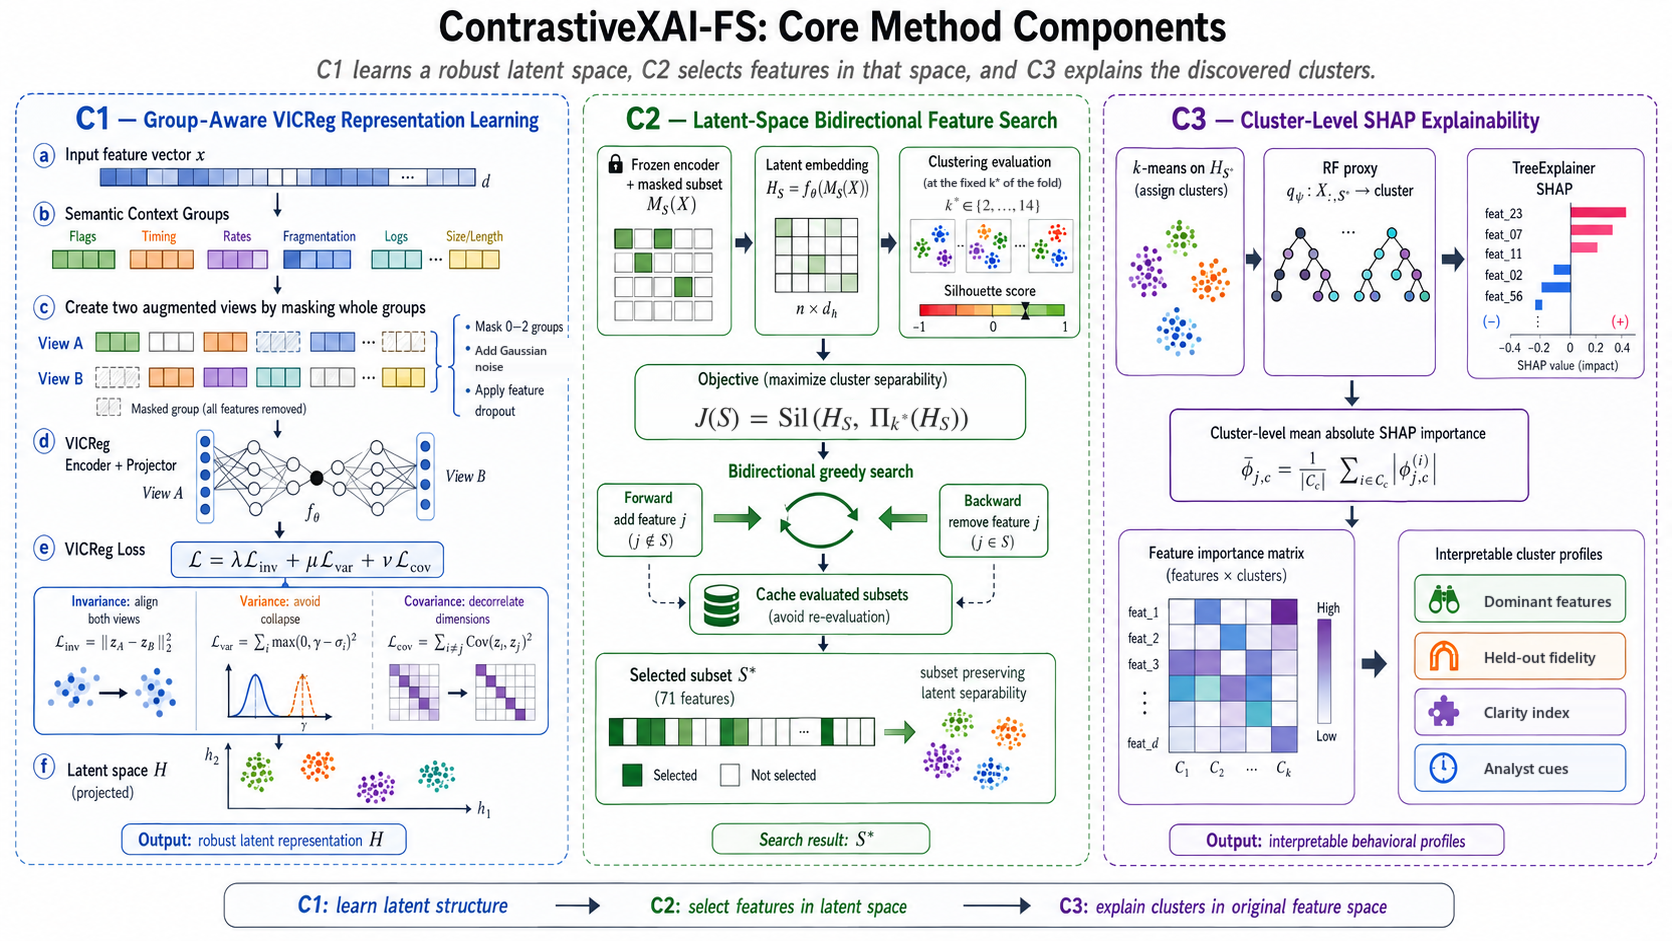
\includegraphics[width=0.95\textwidth]{figures/fig2_pipeline.png}
\caption{Overview of the proposed \method{} pipeline.}
\label{fig:pipeline}
\end{figure*}

\subsection{Group-Aware Semantic Augmentation}
\label{sec:augmentation}

In tabular IIoT traffic, perturbing isolated features can produce semantically inconsistent samples. For example, changing a TCP flag statistic without modifying related flag counts may create an unrealistic protocol state. To reduce this risk, \method{} masks complete semantic Context Groups, while individual feature dropout and Gaussian noise are retained as lower-amplitude complementary perturbations. Let $\mathcal{B} \subseteq \mathcal{G}$ be a set of Context Groups sampled for masking, and let $U(\mathcal{B}) = \bigcup_{G_r \in \mathcal{B}} G_r$ be the union of the feature indices contained in these groups. For each augmented view, the number of masked groups is sampled as
\begin{equation}
m \sim \mathrm{Uniform}\{0, 1, 2\},
\end{equation}
and $m$ groups are then selected uniformly from $\mathcal{G}$ without replacement. The two augmented views of the same sample independently sample their masked groups. Given a standardized input $x$, the augmented view $\tilde{x} = \mathcal{A}(x)$ is defined component-wise as
\begin{equation}
\tilde{x}_j =
\begin{cases}
0, & \text{if } j \in U(\mathcal{B}),\\
r_j\,(x_j + \eta_j), & \text{otherwise},
\end{cases}
\label{eq:augment}
\end{equation}
where $r_j \sim \mathrm{Bernoulli}(1 - p_{\mathrm{drop}})$ is an independent feature-dropout mask with $p_{\mathrm{drop}} = 0.10$ and $\eta_j \sim \mathcal{N}(0, 0.05^2)$ is Gaussian noise expressed in standardized feature units.

Group masking removes a complete semantic observation channel, such as timing, fragmentation, or flag behavior, rather than breaking the internal structure of a group; the Gaussian noise introduces small local variability in the surviving features; and feature dropout prevents the encoder from relying excessively on a small number of individual attributes. The augmentation does not assume that every perturbed vector corresponds to a complete executable network trace. Its purpose is to preserve the relationships among the unmasked measurement contexts while exposing the encoder to controlled uncertainty in the available observations.

\subsection{VICReg Encoder for IIoT Traffic Representation}

\method{} uses VICReg \cite{bardes2022vicreg} to learn a latent representation from unlabeled traffic windows. VICReg is a non-contrastive joint-embedding objective: it does not require negative pairs, and it explicitly penalizes representation collapse through a variance term. This property is useful in IIoT tabular traffic, where the semantic validity of augmentations is more difficult to guarantee than in image-based self-supervised learning.

Let $f_\theta : \mathbb{R}^{d} \rightarrow \mathbb{R}^{p}$ be the encoder and $g_\phi : \mathbb{R}^{p} \rightarrow \mathbb{R}^{r}$ be the projector, with $p = 128$ and $r = 512$. For each sample $x_i$, two augmented views $\tilde{x}_i = \mathcal{A}_1(x_i)$ and $\tilde{x}'_i = \mathcal{A}_2(x_i)$ are generated independently, producing $z_i = g_\phi(f_\theta(\tilde{x}_i))$ and $z'_i = g_\phi(f_\theta(\tilde{x}'_i))$. For a mini-batch of size $b$, let $Z = [z_1,\dots,z_b]^\top$ and $Z' = [z'_1,\dots,z'_b]^\top$. The VICReg loss is
\begin{equation}
\mathcal{L}_{\mathrm{VICReg}} = \lambda\,\mathcal{L}_{\mathrm{inv}}(Z,Z') + \mu\,\mathcal{L}_{\mathrm{var}}(Z,Z') + \nu\,\mathcal{L}_{\mathrm{cov}}(Z,Z').
\label{eq:vicreg}
\end{equation}
The invariance term encourages the two augmented views of the same sample to have similar projections:
\begin{equation}
\mathcal{L}_{\mathrm{inv}}(Z,Z') = \rev{\frac{1}{b\,r}}\sum_{i=1}^{b} \lVert z_i - z'_i \rVert_2^2 .
\end{equation}
The variance term prevents collapse by requiring each projection dimension to maintain sufficient variability within the mini-batch:
\begin{equation}
\mathcal{L}_{\mathrm{var}}(Z,Z') = \rev{\tfrac{1}{2}}\bigl[v(Z) + v(Z')\bigr],
\end{equation}
\begin{equation}
v(Z) = \frac{1}{r}\sum_{j=1}^{r} \max\!\Bigl(0,\; \gamma - \sqrt{\mathrm{Var}(Z_{:,j}) + \epsilon}\Bigr),
\end{equation}
where $\gamma = 1$ is the standard-deviation threshold and $\epsilon = 10^{-4}$ provides numerical stability. The covariance term decorrelates different projection dimensions:
\begin{equation}
\mathcal{L}_{\mathrm{cov}}(Z,Z') = \rev{\tfrac{1}{2}}\bigl[c(Z) + c(Z')\bigr], \qquad
c(Z) = \frac{1}{r}\sum_{i \neq j} [\mathrm{Cov}(Z)]_{ij}^2 ,
\end{equation}
where $\mathrm{Cov}(Z)$ is the empirical covariance matrix of the centered mini-batch projections. \rev{The normalization constants above are those of the implementation used in all experiments.} The weights are set to $\lambda = \mu = 25$ and $\nu = 1$, following the standard VICReg configuration.

The encoder is trained only on the training fold of each cross-validation split. \rev{For computational tractability on the CPU-only platform used in this study, each encoder is trained on a uniform random subsample of at most 20,480 training-fold rows, drawn without reference to labels.} After training, the projector $g_\phi$ is discarded, and only the frozen encoder output $h = f_\theta(x)$ is used for latent-space subset evaluation.

\subsection{Latent-Space Feature Subset Evaluation}
\label{sec:objective}

The method selects original traffic attributes rather than latent dimensions, but each subset of original features is evaluated through the frozen nonlinear representation. This design preserves the physical and operational meaning of the selected inputs while allowing the objective to reflect interactions among traffic measurements that may not be visible from independent feature scores or raw-space distances.

For a candidate subset $S$, unselected features are masked with the operator of Eq.~\eqref{eq:mask}, and the masked data are projected through the frozen encoder:
\begin{equation}
H_S = f_\theta(M_S(X)) \in \mathbb{R}^{n \times p}.
\end{equation}
For a number of clusters $k$, $k$-Means is fitted to $H_S$, producing a partition $\Pi_k(H_S)$ whose quality is measured with the Silhouette score \cite{rousseeuw1987silhouettes}. For each sample $i$, let $a(i)$ be the average distance from $i$ to all other samples in the same cluster, and let $b(i)$ be the smallest average distance from $i$ to the samples of any other cluster. Then
\begin{equation}
s(i) = \frac{b(i) - a(i)}{\max\{a(i), b(i)\}}, \qquad
\Sil(H_S, \Pi_k) = \frac{1}{n}\sum_{i=1}^{n} s(i).
\end{equation}

\rev{The number of clusters is selected once per training fold, using the complete feature set, over the candidate set $\mathcal{K} = \{2,\dots,14\}$:
\begin{equation}
k^{*} = \argmax_{k \in \mathcal{K}} \; \Sil\bigl(H_{[d]}, \Pi_k(H_{[d]})\bigr),
\label{eq:kstar}
\end{equation}
and it is then held fixed during the subset search, so that all candidate subsets are compared at the same partition granularity:
\begin{equation}
J(S) = \Sil\bigl(H_S, \Pi_{k^{*}}(H_S)\bigr).
\label{eq:objective}
\end{equation}
Eqs.~\eqref{eq:kstar} and \eqref{eq:objective} describe the procedure that is actually executed; they replace the per-subset maximization over $k$ stated in the previous version of this manuscript. To keep the search tractable, the objective is estimated on a fixed uniform subsample of the training fold: $k$-Means (five initializations) is fitted on 5,000 training rows, and the Silhouette score is computed on 2,000 of those rows. The same subsample and random seed are used for every candidate subset within a fold, so that $J(S)$ is a deterministic function of $S$.}

Silhouette is used because it provides an internal, label-free measure of cluster cohesion and separation. This criterion does not assume that maximizing Silhouette necessarily maximizes supervised classification performance; the relationship between this objective and downstream detection performance is assessed empirically. A candidate clustering is considered valid only when $k$-Means produces at least two nonempty clusters; invalid configurations are rejected, and subsets containing fewer than two features are not evaluated.

The ideal feature-selection problem, $S^{*} = \argmax_{S \subseteq [d]} J(S)$, cannot be solved exactly because it requires evaluating $2^{d}$ subsets. \method{} therefore uses a bidirectional greedy search that combines backward elimination with forward recovery.

\subsection{Bidirectional Silhouette-Based Search}
\label{sec:search}

The search is initialized with the complete feature set $S_0 = [d]$, which guarantees a valid initial representation. In the backward-removal pass, the algorithm evaluates $S \setminus \{j\}$ for every feature $j \in S$, provided that at least two features remain, and accepts the removal producing the largest strict improvement in $J(S)$. In the forward-recovery pass, it evaluates $S \cup \{j\}$ for every $j \notin S$ and restores the feature whose inclusion produces the largest strict improvement. The procedure alternates these passes until neither a removal nor a reintroduction improves the objective (Algorithm~\ref{alg:search}). All evaluated subsets are stored in a cache that is specific to the current training fold and frozen encoder.

\rev{Because a removal is accepted only when it strictly improves the objective and no cardinality penalty is applied, the search stops at a \emph{natural operating point} whose size is determined by the data. For comparisons at a prescribed cardinality, we use a budget-constrained variant: starting from the natural subset, the feature whose removal leaves the highest $J(S)$ is removed, even when $J$ decreases, until the requested budget is reached. To limit the number of evaluations, $\lfloor 0.1\,|S| \rfloor$ features are removed per pass while $|S| > 25$, and exactly one feature per pass thereafter. The same natural and budget-constrained procedures are applied in the standardized input space for the raw-space $k$-Means+Sil reference.}

\begin{algorithm}[t]
\caption{\method}
\label{alg:main}
\footnotesize
\begin{algorithmic}[1]
\Require Unlabeled training data $X_{\mathrm{tr}}$, Context Groups $\mathcal{G}$, candidate cluster set $\mathcal{K}$
\Ensure Selected subset $S^{*}$, cluster assignments $\hat{y}^{c}$, cluster profiles $\{P_c\}$
\State Fit imputation, infinite-value replacement, and standardization on $X_{\mathrm{tr}}$
\For{each training epoch}
  \For{each mini-batch $B \subset X_{\mathrm{tr}}$}
    \State Generate views $\tilde{B} = \mathcal{A}_1(B)$ and $\tilde{B}' = \mathcal{A}_2(B)$
    \State $Z \gets g_\phi(f_\theta(\tilde{B}))$, \; $Z' \gets g_\phi(f_\theta(\tilde{B}'))$
    \State Update $\theta, \phi$ by minimizing $\mathcal{L}_{\mathrm{VICReg}}(Z, Z')$
  \EndFor
\EndFor
\State Freeze $f_\theta$ and discard $g_\phi$
\State \rev{Select $k^{*}$ with Eq.~\eqref{eq:kstar}}
\State $S^{*} \gets \textsc{BidirectionalSearch}(X_{\mathrm{tr}}, f_\theta, k^{*})$
\State Fit $k$-Means with $k^{*}$ clusters on $H_{S^{*}} = f_\theta(M_{S^{*}}(X_{\mathrm{tr}}))$; obtain $\hat{y}^{c}$
\State \rev{Split the clustered rows into proxy-training and held-out parts}
\State Train Random Forest proxy $q_\psi : X_{:,S^{*}} \rightarrow \hat{y}^{c}$ \rev{on the proxy-training part}
\State \rev{Measure proxy fidelity and compute TreeExplainer SHAP on the held-out part}
\State Compute cluster profiles $\{P_c\}$ \rev{and clarity indices $\{CI_c\}$}
\State \Return $S^{*}$, $\hat{y}^{c}$, $\{P_c\}$
\end{algorithmic}
\end{algorithm}

\begin{algorithm}[t]
\caption{Bidirectional Latent Silhouette Search}
\label{alg:search}
\footnotesize
\begin{algorithmic}[1]
\Require Training data $X$, frozen encoder $f_\theta$, \rev{fixed $k^{*}$}, feature set $[d]$
\Ensure Selected feature subset $S^{*}$
\State $S \gets [d]$; cache $\mathcal{C} \gets \emptyset$; compute and cache $J(S)$
\State $improved \gets$ \textbf{true}
\While{$improved$}
  \State $improved \gets$ \textbf{false}
  \State $S_{\mathrm{best}} \gets S$; $J_{\mathrm{best}} \gets J(S)$ \Comment{Backward-removal pass}
  \For{each feature $j \in S$ with $|S| > 2$}
    \State $S' \gets S \setminus \{j\}$; compute $J(S')$ with Eq.~\eqref{eq:objective} if $S' \notin \mathcal{C}$
    \If{$J(S') > J_{\mathrm{best}}$} $S_{\mathrm{best}} \gets S'$; $J_{\mathrm{best}} \gets J(S')$ \EndIf
  \EndFor
  \If{$S_{\mathrm{best}} \neq S$} $S \gets S_{\mathrm{best}}$; $improved \gets$ \textbf{true} \EndIf
  \State $S_{\mathrm{best}} \gets S$; $J_{\mathrm{best}} \gets J(S)$ \Comment{Forward-recovery pass}
  \For{each feature $j \in [d] \setminus S$}
    \State $S' \gets S \cup \{j\}$; compute $J(S')$ with Eq.~\eqref{eq:objective} if $S' \notin \mathcal{C}$
    \If{$J(S') > J_{\mathrm{best}}$} $S_{\mathrm{best}} \gets S'$; $J_{\mathrm{best}} \gets J(S')$ \EndIf
  \EndFor
  \If{$S_{\mathrm{best}} \neq S$} $S \gets S_{\mathrm{best}}$; $improved \gets$ \textbf{true} \EndIf
\EndWhile
\State \Return $S$
\end{algorithmic}
\end{algorithm}

\subsection{Cluster-Level SHAP Explainability}
\label{sec:xai_method}

The final stage interprets the unsupervised cluster structure produced from the selected feature subset. After selecting $S^{*}$, the data are projected into the selected latent representation, $H_{S^{*}} = f_\theta(M_{S^{*}}(X))$, and a $k$-Means model with $k^{*}$ clusters produces the cluster assignments $\hat{y}^{c}_i \in \{1,\dots,k^{*}\}$.

Because the VICReg encoder is not directly interpretable in terms of original traffic features, we train a Random Forest proxy model $q_\psi$ to reproduce the cluster assignments using only the selected original features:
\begin{equation}
q_\psi : X_{:,S^{*}} \rightarrow \hat{y}^{c}.
\end{equation}
\rev{The proxy explanations describe the relationship between the selected original features and the latent cluster assignments. They do not explain the internal parameters or latent dimensions of the VICReg encoder, nor the sequence of decisions made by the subset search, and they do not establish a one-to-one correspondence between a latent cluster and an attack category. This scope applies to every explainability result reported in this paper and is not repeated in the following sections.}

\rev{To quantify how faithfully the proxy approximates the latent partition, the clustered rows are split, stratified by cluster, into a proxy-training part and a disjoint held-out part. The proxy is fitted on a cluster-balanced sample of the proxy-training part, and its fidelity is measured on the held-out part through accuracy, balanced accuracy, and per-cluster precision, recall, and F1 with respect to the latent cluster assignments. In the cross-validation experiments, fidelity is additionally measured on the outer test fold, whose rows are not seen by the scaler, the encoder, the subset search, the $k$-Means model, or the proxy.}

TreeExplainer SHAP \cite{lundberg2017unified} is then applied to the proxy model \rev{on held-out rows}. For sample $i$, feature $j$, and cluster $c$, the SHAP value $\phi^{(i)}_{j,c}$ estimates the contribution of feature $j$ to the proxy output for cluster $c$. SHAP values are aggregated at the cluster level using the mean absolute contribution,
\begin{equation}
\bar{\phi}_{j,c} = \frac{1}{|\mathcal{C}_c|}\sum_{i \in \mathcal{C}_c} \bigl|\phi^{(i)}_{j,c}\bigr| ,
\label{eq:clustershap}
\end{equation}
where $\mathcal{C}_c$ is the set of \rev{held-out} samples assigned to cluster $c$, and the behavioral profile of a cluster is the set of its top-$M$ features according to $\bar{\phi}_{j,c}$. Because the Context Groups contain different numbers of features, raw group-level SHAP sums are not used for cross-group ranking; the analysis relies on feature-level contributions.

\rev{Not every cluster yields a profile that an analyst can read. To avoid a subjective choice of which clusters to interpret, each cluster receives a \emph{clarity index}
\begin{equation}
CI_c = F_c \cdot T_c, \qquad
T_c = \frac{\sum_{j \in \mathrm{Top3}(c)} \bar{\phi}_{j,c}}{\sum_{j \in S^{*}} \bar{\phi}_{j,c}},
\label{eq:clarity}
\end{equation}
where $F_c$ is the held-out F1 of the proxy for cluster $c$ and $T_c$ is the share of the cluster's SHAP mass carried by its three most important features. $F_c$ measures whether the explanation is faithful to the latent cluster, and $T_c$ measures whether the profile is concentrated enough to be summarized by a few attributes. The index is reported for all clusters, and detailed interpretation is given in decreasing order of $CI_c$.}

\subsection{Computational Complexity and Scalability}
\label{sec:complexity}

The computational cost is divided into VICReg training, candidate-subset evaluation, and post-hoc proxy interpretation. Let $E$ denote the number of training epochs, \rev{$n_e$ the number of rows used for encoder training}, and $P$ the number of trainable parameters in the encoder and projector. For the fully connected architecture used here, representation learning costs approximately $O(E\,n_e\,P)$.

After training, the encoder is frozen. \rev{For one candidate subset, with $n_s$ rows used for clustering and $n_v \le n_s$ rows used for the Silhouette estimate, masking and encoding cost $O(n_s d + n_s P_f)$, where $P_f$ is the size of the frozen encoder; $k$-Means with $I$ iterations costs $O(I\,n_s\,p\,k^{*})$; and the Silhouette estimate costs $O(n_v^{2}\,p)$. One backward pass evaluates at most $|S|$ candidates and one forward-recovery pass at most $d - |S|$. If $T$ unique subsets are evaluated before convergence, the search costs $O\bigl(T\,(n_s d + n_s P_f + I\,n_s\,p\,k^{*} + n_v^{2}\,p)\bigr)$.} The cache ensures that each unique candidate is scored at most once within a fold. Increasing $d$ enlarges the number of neighboring subsets examined at each pass, whereas the subsampling makes the per-candidate cost independent of the training-fold size. \rev{The measured offline cost of these stages on the experimental platform is reported in Section~\ref{sec:cost}.}

\section{Experimental Setup}
\label{sec:setup}

The evaluation is designed to answer \rev{seven} questions: (i) whether the selected features preserve downstream intrusion-detection performance; (ii) whether the method is competitive with classical unsupervised feature-selection baselines; (iii) how each method behaves under fixed feature budgets; (iv) whether the learned clusters can be interpreted through the original traffic features; \rev{(v) how stable the selected subsets, the selected number of clusters, and the clusters themselves are across folds and independent master seeds; (vi) how the conclusions change when related traffic windows are kept out of the test partition; and (vii) whether the pipeline can be applied to other IoT/IIoT datasets with different feature schemas.}

\subsection{Cross-Validation and Anti-Leakage Protocol}
\label{sec:cv}

The main experiments use 10-fold stratified cross-validation. \rev{The folds are stratified by the eight-class label \feat{label2}; because benign traffic is one of the eight classes, the same partition is also stratified with respect to the binary label and is used for both tasks.} The labels are used only to construct the outer evaluation folds and to compute downstream metrics. They are not provided to the scaler, VICReg encoder, clustering algorithm, Silhouette objective, feature-selection search, or SHAP proxy.

For each fold $r$, with training and test sets $X^{(r)}_{\mathrm{tr}}$ and $X^{(r)}_{\mathrm{te}}$, the processing order is: training-fold imputation and standardization, VICReg training, selection of $k^{*}_r$, latent-space feature selection, downstream classifier fitting, and test-fold evaluation. The scaler, encoder, clustering structure, subset-search cache, and selected subset $S^{*}_r$ are recomputed within each fold and are not transferred from another fold; downstream classifiers are trained on $X^{(r)}_{\mathrm{tr},:,S^{*}_r}$ and evaluated on $X^{(r)}_{\mathrm{te},:,S^{*}_r}$. \rev{All unsupervised baselines follow the same rule. Every number reported in Section~\ref{sec:results} was produced by this fold-internal implementation, which is released with the paper.}

\rev{\textbf{Sample-level folds.} In the main protocol the folds are generated at the level of individual one-second windows. Windows from the same device, attack execution, or temporal neighborhood can therefore be assigned to both the training and the test partition. In addition, 35.3\% of the test windows have an exact duplicate in the corresponding training partition; almost all of these are the idle windows described in Section~\ref{sec:dataset}, and only \DupNonIdle\% of the test windows are non-idle exact duplicates. The sample-level results must consequently be read as within-dataset IID generalization.}

\rev{\textbf{Grouped folds.} To measure how much the sample-level protocol benefits from related windows, the complete pipeline is also executed under two grouped protocols, each with five stratified folds. In the \emph{execution-grouped} protocol, a group is one attack execution (one value of \feat{label_full}) or, for benign traffic, one contiguous 60-s block of the benign capture shared by all devices; all windows of an attack execution and all windows of a benign time block are therefore assigned to the same fold. In the \emph{device-grouped} protocol, the group is the device identity, so that the test partition contains only devices that were never seen during scaling, encoder training, feature selection, or classifier fitting. Because web attacks are recorded on a single device and brute-force attempts on five devices, some categories are absent from the training partition of some device-grouped folds; the affected classes are reported explicitly.}

\subsection{Independent Master Seeds}
\label{sec:seeds}

\rev{The complete 10-fold experiment is executed three times with independent master seeds $s \in \{42, 43, 44\}$. The master seed determines the outer-fold partition, and the derived seed $s + r$ initializes every stochastic component of fold $r$: the encoder-training subsample, neural-network initialization, mini-batch order, augmentation sampling, the subsample used by the Silhouette objective, $k$-Means initialization, the graph subsamples of the spectral baselines, and the Random Forest and Decision Tree classifiers. The three executions therefore differ in the data partition and in all sources of randomness. Results are reported per seed and across seeds, and the 30 fold-specific subsets are used for the stability analysis. Seed 42 is the primary execution: it includes all baselines, the KNN classifier, and the fixed-budget regime, whereas seeds 43 and 44 evaluate \method{} and the All Features reference with Random Forest and Decision Tree. The number of seeds was limited to three, the lower end of the usual range, by the CPU-only platform.}

\subsection{Evaluation Tasks and Regimes}

Two intrusion-detection tasks are evaluated: a binary task based on \feat{label1} and an eight-class task based on \feat{label2}. In both tasks, the target labels are introduced only after the unsupervised feature-selection stage.

Feature-selection methods are evaluated under two regimes. In the \emph{natural operating point} regime, each method determines its own subset size; results obtained with different numbers of features are distinct operating points and are not matched-budget comparisons. In the \emph{constrained feature-budget} regime, all methods retain exactly $k \in \{10, 15, 20, 25\}$ features; this regime provides the matched-cardinality comparison. Ranking-based methods select their top-$k$ features. \rev{Subset-search methods (\method{} and $k$-Means+Sil) use the budget-constrained variant defined in Section~\ref{sec:search}.}

\subsection{Downstream Classifiers}

Classification performance is evaluated using Random Forest (RF, 100 trees), Decision Tree (DT, Gini criterion), and $k$-Nearest Neighbors (KNN, $k = 5$). RF is an ensemble that is robust to noisy features, DT is more sensitive to spurious split candidates, and KNN evaluates whether the selected subset preserves neighborhood structure. The same classifier configuration is used for all methods within each fold, without hyperparameter tuning. The classifiers do not participate in the Silhouette objective or in the selection of $S^{*}_r$.

\subsection{Metrics and Statistical Testing}

The primary metric is macro-F1, the unweighted average of the per-class F1 scores,
\begin{equation}
F1_{\mathrm{macro}} = \frac{1}{C}\sum_{c=1}^{C} \frac{2\,\mathrm{Precision}_c\,\mathrm{Recall}_c}{\mathrm{Precision}_c + \mathrm{Recall}_c},
\end{equation}
where $C$ is the number of classes. Secondary metrics are accuracy, macro-precision, macro-recall, and the Matthews correlation coefficient (MCC).

Statistical significance is assessed with the two-sided Wilcoxon signed-rank test over paired folds: the score of \method{} in a fold is compared with the score of the reference method on the same training and test partitions. \rev{Two-sided $p$-values are reported throughout. Tests are reported for the primary execution (10 pairs) and for the three executions pooled (30 pairs); folds from different master seeds partition the same dataframe and are therefore not independent samples, so the pooled test is interpreted together with the sign and size of the differences.} A non-significant result is not treated as evidence of equivalence.

\rev{\textbf{Selection stability.} For the fold-specific subsets we report the distribution of subset sizes, the selection frequency of every feature, the pairwise Jaccard similarity $|S_a \cap S_b| / |S_a \cup S_b|$ between subsets, and the stability estimator of Nogueira \emph{et al.} \cite{nogueira2018stability}, which corrects for chance agreement and accommodates subsets of different sizes (1 indicates identical subsets; 0 corresponds to random selection of the same average size). Because most features are retained, the Jaccard similarity of the \emph{removed} sets is also reported; it is the more demanding measure.}

\rev{\textbf{Cluster stability.} Two measures are reported, both using the adjusted Rand index (ARI) \cite{hubert1985comparing} and the adjusted mutual information (AMI) \cite{vinh2010information}. \emph{Within-fold} stability refits $k$-Means on five independently drawn training-fold subsamples with different initializations and compares the labels assigned to a common reference subsample. \emph{Cross-pipeline} stability lets every fold-specific pipeline (scaler, encoder, selected subset, and $k$-Means centers) label the same 5,000 fixed reference windows and compares all pairs of pipelines, within and across master seeds; it therefore includes the variability of encoder training and feature selection.}

\subsection{Baseline and Reference Methods}

The evaluated unsupervised methods are:
\begin{itemize}
\item \textbf{Variance ranking}: top-$k$ features with the largest training-fold variance. \rev{Because the variance of every $z$-scored feature equals one, the variance is computed after min--max scaling with training-fold statistics.}
\item \textbf{Laplacian Score} \cite{he2005laplacian}: ranks features by their locality-preserving ability with respect to a nearest-neighbor graph.
\item \textbf{SPEC} \cite{zhao2007spectral}: evaluates features using a spectral graph objective.
\item \textbf{MCFS} \cite{cai2010unsupervised}: selects features through sparse regression over spectral embeddings.
\item \textbf{UDFS} \cite{yang2011l2} and \textbf{NDFS} \cite{li2012unsupervised}: structured-sparsity and nonnegative spectral selection.
\item \textit{k}\textbf{-Means+Sil}: the same \rev{$k^{*}$ selection,} bidirectional search\rev{, and budget-constrained variant as \method{}, applied in the standardized original feature space instead of the VICReg latent space. It isolates the effect of the evaluation space.}
\end{itemize}
\rev{The graph-based methods use a 5-nearest-neighbor graph built on 5,000 training-fold rows, and MCFS uses five spectral components.} At their natural operating point, the ranking methods retain 25 features.

Two reference configurations are also included. \emph{All Features} uses all numeric features and serves as a no-selection reference. \emph{DataSense-17} (DS-17) \cite{firouzi2025datasense} is the compact subset reported with the dataset; because it was obtained with label information, it is treated as a fixed external supervised reference, is not re-selected within the folds, and is not ranked as an unsupervised baseline.

\subsection{Controlled Component Comparisons}
\label{sec:ablation_setup}

\rev{Three controlled comparisons are added in which exactly one component is changed while the folds, seeds, encoder architecture, optimization schedule, objective, and search are held fixed. (a) \emph{Augmentation}: the group-aware encoder is compared with an encoder trained with independent per-feature masking at the same expected masking rate ($E[m]/q = 1/9$ of the features per view, the standard unstructured corruption used by SCARF-like methods \cite{bahri2022scarf}), with identical Gaussian noise and feature dropout. (b) \emph{Search direction}: the bidirectional search is compared with a backward-only search on the same encoder and objective. (c) \emph{Evaluation space}: the latent-space and raw-space searches are compared at identical feature budgets and at the cardinality of the latent natural subset. Comparisons (b) and (c) use all ten folds of the primary execution; comparison (a) requires retraining the encoder and uses its first five folds.}

\subsection{Additional Datasets: N-BaIoT and WUSTL-IIoT-2021}
\label{sec:wustl_setup}

\rev{To examine whether the pipeline can be applied beyond DataSense, the complete fold-wise protocol is repeated on two public IoT/IIoT datasets with schemas that differ from DataSense. The encoder, subsets, and classifiers are trained and tested within each dataset, so these experiments assess the applicability of the unchanged method to new schemas with dataset-specific Context Groups rather than transfer of a trained model across datasets. No hyperparameter of Table~\ref{tab:config} was tuned on either dataset. The ranking baselines retain 35\% of the features at their natural operating point, the same proportion as the 25 of 71 features used for DataSense. Both datasets consist of flow statistics with heavy-tailed magnitudes (packet counts, byte counts, and variances spanning several orders of magnitude); for both, a stateless signed log transform $x \mapsto \mathrm{sign}(x)\log(1+|x|)$ is applied to every attribute before the fold-wise standardization, a decision taken from the label-free marginal distributions. The evaluation protocol, the compared configurations, and the statistical decision rules for the N-BaIoT experiment were registered in the public repository before the experiment was run.}

\rev{\textbf{N-BaIoT} \cite{meidan2018n} contains traffic of nine commercial IoT devices (doorbells, a thermostat, a baby monitor, and security cameras) infected by the Mirai and BASHLITE (Gafgyt) botnets. Each record has 115 numeric statistics computed over five damped time windows for five stream aggregations: source MAC-IP, source IP, channel, channel jitter, and socket. These five stream aggregations define its Context Groups (15, 15, 35, 15, and 35 features). A uniform label-free sample of 3.5\% of the 7,062,606 records is drawn once (247,277 records), and a binary task and an eleven-class task (benign traffic and five attacks of each botnet) are evaluated, with fixed budgets $k \in \{10, 20, 30, 40\}$.}

\rev{\textbf{WUSTL-IIoT-2021}} \rev{is evaluated next. The complete fold-wise protocol is applied to WUSTL-IIoT-2021 \cite{zolanvari2021wustl,zolanvari2019machine}, a public dataset collected from an industrial control testbed (SCADA and Modbus traffic among PLCs, sensors, and actuators) that contains normal traffic and denial-of-service, reconnaissance, command-injection, and backdoor attacks. It was chosen because it is an IIoT dataset rather than a consumer-IoT dataset, is directly downloadable, consists of numeric tabular attributes, and has a schema that differs substantially from DataSense: its samples are bidirectional flow records rather than per-device one-second windows, it has no device-log attributes and no fragmentation or address-diversity counters, and it is strongly imbalanced (92.7\% normal traffic).}

\rev{Following the recommendation of the dataset authors, the columns \feat{StartTime}, \feat{LastTime}, \feat{SrcAddr}, \feat{DstAddr}, \feat{sIpId}, and \feat{dIpId} are removed, which leaves 41 numeric attributes. To keep the cost comparable with DataSense, a uniform random sample of 25\% of the 1,194,464 flows is drawn once, without reference to labels (298,616 flows: 276,622 normal, 19,856 DoS, 2,018 reconnaissance, 63 command injection, and 57 backdoor). A binary task and a five-class task are evaluated with RF and DT.}

\rev{The Context Groups cannot be transferred from DataSense and were rebuilt with the construction rule of Section~\ref{sec:groups}, using only the documented meaning of each flow attribute (Table~\ref{tab:wustl_groups}). The ranking baselines retain 14 features, and the fixed budgets are $k \in \{5, 10, 15, 20\}$.}

\begin{table}[t]
\revon
\caption{Context Groups Rebuilt for WUSTL-IIoT-2021 (41 Flow Attributes)}
\label{tab:wustl_groups}
\centering
\footnotesize
\begin{tabular}{@{}p{2.55cm}cp{4.6cm}@{}}
\toprule
Context Group & \# & Attributes \\
\midrule
Flow Duration and Activity & 7 & \feat{Dur}, \feat{RunTime}, \feat{Mean}, \feat{Sum}, \feat{Min}, \feat{Max}, \feat{IdleTime} \\
Packet/Byte Volume & 6 & \feat{SrcPkts}, \feat{DstPkts}, \feat{TotPkts}, \feat{SrcBytes}, \feat{DstBytes}, \feat{TotBytes} \\
Traffic Rate and Load & 6 & \feat{SrcLoad}, \feat{DstLoad}, \feat{Load}, \feat{SrcRate}, \feat{DstRate}, \feat{Rate} \\
Inter-Packet Timing and Jitter & 6 & \feat{SrcJitter}, \feat{DstJitter}, \feat{SIntPkt}, \feat{DIntPkt}, \feat{SrcJitAct}, \feat{DstJitAct} \\
Loss and Retransmission & 4 & \feat{SrcLoss}, \feat{DstLoss}, \feat{Loss}, \feat{pLoss} \\
IP Header Control & 4 & \feat{sTtl}, \feat{dTtl}, \feat{sTos}, \feat{sDSb} \\
Application Payload & 3 & \feat{SAppBytes}, \feat{DAppBytes}, \feat{TotAppByte} \\
Network Multiplexing & 3 & \feat{Proto}, \feat{Sport}, \feat{Dport} \\
Connection Setup & 2 & \feat{TcpRtt}, \feat{SynAck} \\
\bottomrule
\end{tabular}
\end{table}

\subsection{Encoder and Search Configuration}

Table~\ref{tab:config} summarizes the configuration. The encoder maps the standardized feature vector to a 128-dimensional latent representation, and the projector maps it to a 512-dimensional space used only during VICReg training. The projector is intentionally wider than the encoder output, following the standard VICReg design in which the projection space absorbs the constraints imposed by the loss terms. The Random Forest proxy is fitted only after the latent clusters have been constructed and does not participate in VICReg training, feature selection, or downstream attack classification; its agreement with the latent cluster assignments is distinct from the intrusion-detection metrics.

\begin{table}[t]
\caption{\method{} Hyperparameters and Experimental Configuration}
\label{tab:config}
\centering
\footnotesize
\setlength{\tabcolsep}{3pt}
\begin{tabular}{@{}p{1.55cm}p{2.35cm}p{4.3cm}@{}}
\toprule
Component & Parameter & Value \\
\midrule
Input & Numeric features & 71 (DataSense); \rev{41 (WUSTL-IIoT-2021)} \\
 & Preprocessing & Training-fold imputation and standardization \\
 & Context Groups & 9 semantic groups \rev{per dataset} \\
Encoder $f_\theta$ & Architecture & $d{\rightarrow}256$(BN, ReLU, Dropout 0.2)${\rightarrow}128$(BN, ReLU) \\
Projector $g_\phi$ & Architecture & $128{\rightarrow}512$(BN, ReLU)${\rightarrow}512$ \\
VICReg & $(\lambda, \mu, \nu)$; $\gamma$; $\epsilon$ & $(25, 25, 1)$; $1.0$; $10^{-4}$ \\
Optimization & Optimizer & AdamW, learning rate $10^{-3}$, weight decay $10^{-4}$ \\
 & Scheduler & Cosine annealing, $\eta_{\min} = 10^{-5}$ \\
 & Epochs / batch size & 100 / 512 \\
 & Gradient clipping & Maximum norm 1.0 \\
 & \rev{Training rows} & \rev{Uniform subsample of $\le$20,480 training-fold rows} \\
Augmentation & Group masking & $m \sim \mathrm{Uniform}\{0,1,2\}$ groups \\
 & Gaussian noise & $\mathcal{N}(0, 0.05^{2})$ in standardized units \\
 & Feature dropout & $p_{\mathrm{drop}} = 0.10$ \\
Feature search & Cluster range & $\mathcal{K} = \{2,\dots,14\}$ \\
 & Objective & Latent Silhouette at \rev{fold-specific $k^{*}$ (Eq.~\ref{eq:objective})} \\
 & \rev{Objective estimate} & \rev{$k$-Means on 5,000 training rows (5 initializations); Silhouette on 2,000 rows} \\
 & Direction & Backward removal with forward recovery \\
 & Initialization & Complete feature set; minimum size 2 \\
 & \rev{Budget variant} & \rev{Forced backward elimination (Sec.~\ref{sec:search})} \\
Classifiers & RF / DT / KNN & 100 trees / Gini / $k = 5$ \\
SHAP proxy & Model & Random Forest, 200 trees, depth 10 \\
 & \rev{Training sample} & \rev{Cluster-balanced, $\le$5,000 rows; fidelity and SHAP on held-out rows} \\
Reproducibility & \rev{Master seeds} & \rev{42, 43, 44 (fold seed $s + r$)} \\
 & \rev{Repetitions} & \rev{Three complete 10-fold executions} \\
 & Platform & Dell XPS 9320, Intel Core i7-1260P, Windows 11, \rev{CPU only} \\
\bottomrule
\end{tabular}
\end{table}

\subsection{Reproducibility}
\label{sec:repro}

Whenever a method requires the number of clusters as an internal parameter, the value is selected using only the training fold. Identical fold assignments across methods preserve the paired structure of the comparisons. The experiments were executed on a Dell XPS 9320 notebook running Microsoft Windows 11 and equipped with a 12th-generation Intel Core i7-1260P processor with 12 cores and 16 logical processors, \rev{without GPU acceleration. The implementation, the fold-wise runner, the configuration, the per-fold selected subsets, and the scripts that generate every table and figure of Section~\ref{sec:results} are described in the Data and Code Availability statement.}

\section{Results}
\label{sec:results}

This section reports feature-selection quality and its stability across folds and seeds (§\ref{sec:res_selection}), downstream classification performance (§\ref{sec:res_classification}), robustness under fixed feature budgets (§\ref{sec:res_budget}), controlled component comparisons (§\ref{sec:res_ablation}), grouped evaluation protocols (§\ref{sec:res_grouped}), additional datasets (§\ref{sec:res_external}), and SHAP-based cluster explainability (§\ref{sec:res_xai}). \rev{Unless otherwise stated, results refer to the primary execution (master seed 42) and are reported as mean values across its 10 folds.}

\subsection{Feature Selection Quality and Stability}
\label{sec:res_selection}

\rev{Because feature selection is performed independently in every training fold, each fold produces its own subset $S^{*}_r$. Table~\ref{tab:stability} summarizes the 30 fold-specific subsets obtained with the three master seeds, and Fig.~\ref{fig:selfreq} shows the selection frequency of every feature that was removed at least once. The subsets retain a median of 61 features (mean 55.7), and the pairwise Jaccard similarity between subsets is 0.69, both within a seed (0.70) and across seeds (0.69), which is substantially higher than for the raw-space $k$-Means+Sil wrapper (0.40). Forty-six of the 71 features are selected in at least 80\% of the folds.}

\rev{The features that are removed most often form a coherent group: the four inter-packet timing statistics \feat{network_time-delta_avg}, \feat{network_time-delta_max}, \feat{network_time-delta_min}, and \feat{network_time-delta_std_deviation} are removed in 67--73\% of the folds, followed by \feat{network_interval-packets} and several log-derived range statistics. TTL, TCP window-size, and most header-flag and size statistics are retained in nearly every fold. This pattern is consistent with the descriptive configuration discussed in Section~\ref{sec:res_xai} and with the interpretation that inter-packet timing in IIoT traffic largely reflects device polling and reporting cycles.}

\begin{table*}[t]
\revon
\caption{Stability of the Fold-Specific Feature Subsets}
\label{tab:stability}
\centering
\footnotesize
\begin{tabular}{@{}lcccccccc@{}}
\toprule
Selector (dataset) & Folds & Mean $|S^{*}_r|$ & Range & Always selected & Never selected & Jaccard (selected) & Jaccard (removed) & Nogueira stability \\
\midrule
\method{} (DataSense) & 30 & 55.7 & 13--70 & 5 & 0 & 0.692 & 0.190 & 0.185 \\
$k$-Means+Sil (DataSense) & 10 & 35.9 & 7--63 & 3 & 6 & 0.404 & 0.417 & 0.174 \\
\method{} (N-BaIoT) & 10 & 74.2 & 35--107 & 15 & 1 & 0.565 & 0.327 & 0.241 \\
$k$-Means+Sil (N-BaIoT) & 10 & 87.1 & 21--114 & 20 & 0 & 0.662 & 0.227 & 0.192 \\
\method{} (WUSTL-IIoT) & 10 & 15.6 & 3--35 & 0 & 4 & 0.336 & 0.514 & 0.191 \\
$k$-Means+Sil (WUSTL-IIoT) & 10 & 11.0 & 2--32 & 0 & 9 & 0.313 & 0.640 & 0.202 \\
\bottomrule
\multicolumn{9}{@{}p{0.97\textwidth}@{}}{Jaccard values are means over all pairs of folds. ``Always''/``Never'' count the features selected in all/none of the folds. DataSense, N-BaIoT, and WUSTL-IIoT-2021 have 71, 115, and 41 features, respectively. The \method{} rows for DataSense pool the three master seeds; the other rows use the primary execution.}
\end{tabular}
\end{table*}


\begin{figure}[t]
\centering
\includegraphics[width=\columnwidth]{figures/fig_selection_frequency_datasense.pdf}
\caption{\rev{Selection frequency over the 30 fold-specific subsets (three master seeds) of the DataSense features that are selected in fewer than 80\% of the folds. The remaining 46 features are selected in at least 80\% of the folds.}}
\label{fig:selfreq}
\end{figure}

\rev{\textbf{Number of clusters.} Fig.~\ref{fig:silprofile} reports the latent Silhouette profile over the candidate set $\mathcal{K} = \{2,\dots,14\}$. The profile rises steeply up to $k \approx 10$ and then flattens, and the selected value lies at the upper end of the candidate range in all folds ($k^{*} = 14$ in 23 folds, 13 in 5, and 12 or 11 in one fold each); in the descriptive configuration, $k^{*} = 13$ (Silhouette 0.554, versus 0.552 at $k = 14$). Extending the profile beyond the candidate range (Fig.~\ref{fig:silext}) shows a slow further increase, from 0.567 at $k = 14$ to 0.622 at $k = 30$. The upper bound of $\mathcal{K}$ therefore acts as the granularity limit of the explanation: it keeps the number of cluster profiles small enough to be inspected by an analyst while operating on the plateau of the Silhouette curve. The selected subsets also raise the mean latent Silhouette at every candidate $k$ (Fig.~\ref{fig:silprofile}), confirming that the search improves latent separability independently of the particular value of $k$.}

\begin{figure}[t]
\centering
\includegraphics[width=\columnwidth]{figures/fig_silhouette_profile_datasense.pdf}
\caption{\rev{Latent Silhouette profile over the candidate cluster numbers (mean $\pm$ standard deviation over the 30 fold-specific pipelines), for the complete feature set and for the selected subset $S^{*}_r$.}}
\label{fig:silprofile}
\end{figure}

\begin{figure}[t]
\centering
\includegraphics[width=\columnwidth]{figures/fig_silhouette_extended_datasense.pdf}
\caption{\rev{Latent Silhouette of the complete feature set for $k = 2,\dots,30$ (10 folds of the primary execution). The shaded region is the candidate set used by the search.}}
\label{fig:silext}
\end{figure}

\subsection{Classification Performance}
\label{sec:res_classification}

Table~\ref{tab:natural} reports classification results averaged across RF, DT, and KNN. The methods retain different numbers of features, so the table presents the natural operating point of each configuration and must be read together with the \#F column; equal-cardinality comparisons are reported in Section~\ref{sec:res_budget}.

\begin{table}[t]
\revon
\caption{Classification Results on DataSense at the Natural Operating Point of Each Method (Mean$\pm$Std Over 10 Folds, Master Seed 42, Average of RF/DT/KNN)}
\label{tab:natural}
\centering
\footnotesize
\setlength{\tabcolsep}{3pt}
\begin{tabular}{@{}llccccc@{}}
\toprule
Method & \#F & Bin.\ F1 & 8-cl. F1 & Acc. & MCC & Recall \\
\midrule
\method & 59.2 (28--70) & .931\,{\scriptsize$\pm$.003} & .886\,{\scriptsize$\pm$.005} & .927 & .877 & .840 \\
$k$-Means+Sil & 35.9 (7--63) & .885\,{\scriptsize$\pm$.082} & .732\,{\scriptsize$\pm$.238} & .874 & .776 & .695 \\
MCFS & 25 & .926\,{\scriptsize$\pm$.002} & .861\,{\scriptsize$\pm$.002} & .915 & .856 & .816 \\
Variance & 25 & .932\,{\scriptsize$\pm$.001} & .889\,{\scriptsize$\pm$.004} & .928 & .878 & .842 \\
SPEC & 25 & .931\,{\scriptsize$\pm$.003} & .847\,{\scriptsize$\pm$.021} & .916 & .858 & .809 \\
Laplacian & 25 & .933\,{\scriptsize$\pm$.002} & .810\,{\scriptsize$\pm$.022} & .903 & .835 & .770 \\
NDFS & 25 & .923\,{\scriptsize$\pm$.006} & .821\,{\scriptsize$\pm$.021} & .905 & .839 & .775 \\
UDFS & 25 & .917\,{\scriptsize$\pm$.010} & .843\,{\scriptsize$\pm$.024} & .912 & .850 & .794 \\
\midrule
All Features & 71 & .929\,{\scriptsize$\pm$.001} & .883\,{\scriptsize$\pm$.002} & .925 & .873 & .839 \\
DS-17$^{\dagger}$ & 17 & .919\,{\scriptsize$\pm$.002} & .851\,{\scriptsize$\pm$.004} & .913 & .852 & .807 \\
\bottomrule
\multicolumn{7}{@{}p{0.97\columnwidth}@{}}{\#F: mean number of selected features over the folds (range in parentheses when the size varies). Acc., MCC, and Recall refer to the 8-class task. Different \#F values are different operating points, not a matched-budget ranking. $^{\dagger}$Supervised reference subset.}
\end{tabular}
\end{table}


\rev{With Random Forest, \method{} reaches 0.936 binary and 0.908 eight-class macro-F1, against 0.936 and 0.911 for All Features. Table~\ref{tab:wilcoxon} reports the paired tests. A two one-sided equivalence test with a margin of $\pm$0.01 macro-F1 confirms that \method{} is statistically equivalent to the all-feature configuration in both tasks and with both RF and DT. \method{} significantly outperforms MCFS-25 with RF in both tasks (+0.0018 binary and +0.0072 eight-class; $p = 0.020$ and $p = 0.014$) and with DT in the eight-class task ($p = 0.002$), and it outperforms the supervised DS-17 reference in all folds of both tasks ($p = 0.002$). With the distance-based KNN classifier, the selected subset improves eight-class macro-F1 from 0.839 to 0.851 relative to All Features, which is consistent with the removal of attributes that do not contribute to the neighborhood structure.}

\begin{table}[t]
\revon
\caption{Paired Comparisons of \method{} With Reference Configurations (Two-Sided Wilcoxon Signed-Rank Test Over Folds)}
\label{tab:wilcoxon}
\centering
\footnotesize
\setlength{\tabcolsep}{2.5pt}
\begin{tabular}{@{}lllrcrrcr@{}}
\toprule
 & & & \multicolumn{3}{c}{Seed 42 (10 folds)} & \multicolumn{3}{c}{Seeds 42--44 (30 folds)} \\
\cmidrule(lr){4-6}\cmidrule(l){7-9}
Task & Clf. & Reference & $\Delta$F1 & Wins & $p$ & $\Delta$F1 & Wins & $p$ \\
\midrule
Binary & RF & vs. All Features & -0.0009 & 4/10 & 0.193 & -0.0021 & 7/30 & $<$0.001 \\
Binary & RF & vs. DS-17 & +0.0093 & 10/10 & 0.002 & -- & -- & -- \\
Binary & RF & vs. $k$-Means+Sil & +0.0478 & 10/10 & 0.002 & -- & -- & -- \\
Binary & RF & vs. MCFS-25 & +0.0018 & 8/10 & 0.020 & -- & -- & -- \\
Binary & DT & vs. All Features & -0.0001 & 3/10 & 0.557 & -0.0009 & 13/30 & 0.382 \\
Binary & DT & vs. DS-17 & +0.0123 & 10/10 & 0.002 & -- & -- & -- \\
Binary & DT & vs. $k$-Means+Sil & +0.0469 & 7/10 & 0.084 & -- & -- & -- \\
Binary & DT & vs. MCFS-25 & +0.0032 & 9/10 & 0.004 & -- & -- & -- \\
\midrule
8-class & RF & vs. All Features & -0.0027 & 2/10 & 0.049 & -0.0089 & 6/30 & $<$0.001 \\
8-class & RF & vs. DS-17 & +0.0312 & 10/10 & 0.002 & -- & -- & -- \\
8-class & RF & vs. $k$-Means+Sil & +0.1605 & 9/10 & 0.010 & -- & -- & -- \\
8-class & RF & vs. MCFS-25 & +0.0072 & 9/10 & 0.014 & -- & -- & -- \\
8-class & DT & vs. All Features & -0.0004 & 6/10 & 0.625 & -0.0053 & 19/30 & 0.570 \\
8-class & DT & vs. DS-17 & +0.0381 & 10/10 & 0.002 & -- & -- & -- \\
8-class & DT & vs. $k$-Means+Sil & +0.1566 & 7/10 & 0.064 & -- & -- & -- \\
8-class & DT & vs. MCFS-25 & +0.0147 & 10/10 & 0.002 & -- & -- & -- \\
\bottomrule
\multicolumn{9}{@{}p{0.97\columnwidth}@{}}{$\Delta$F1: mean macro-F1 of \method{} minus the reference. Wins: folds in which \method{} is strictly higher. The $k$-Means+Sil, MCFS-25, and DS-17 configurations were evaluated only in the primary execution.}
\end{tabular}
\end{table}


\rev{\textbf{Independent master seeds.} Table~\ref{tab:seeds} reports three complete executions of the 10-fold experiment with master seeds 42, 43, and 44. Across seeds, \method{} reaches $0.935 \pm 0.001$ binary and $0.902 \pm 0.005$ eight-class RF macro-F1 (mean $\pm$ standard deviation of the seed means). Over the 30 paired folds, the difference to All Features remains within the equivalence margin in both tasks (equivalence test $p < 0.001$ binary and $p = 0.015$ eight-class with RF; $p < 0.001$ and $p = 0.001$ with DT).}

\begin{table*}[t]
\revon
\caption{Three Independent Executions of the Complete 10-Fold Experiment (Macro-F1; Per-Seed Entries: Mean$\pm$Std Over the 10 Folds; Last Row: Mean$\pm$Std of the Three Seed Means)}
\label{tab:seeds}
\centering
\footnotesize
\begin{tabular}{@{}lcccccccc@{}}
\toprule
 & & & \multicolumn{2}{c}{Binary, RF} & \multicolumn{2}{c}{8-class, RF} & \multicolumn{2}{c}{8-class, DT} \\
\cmidrule(lr){4-5}\cmidrule(lr){6-7}\cmidrule(l){8-9}
Master seed & $|S^{*}_r|$ mean (range) & $k^{*}_r$ range & \method & All Features & \method & All Features & \method & All Features \\
\midrule
42 & 59.2 (28--70) & 13--14 & .936\,{\scriptsize$\pm$.002} & .936\,{\scriptsize$\pm$.001} & .908\,{\scriptsize$\pm$.005} & .911\,{\scriptsize$\pm$.003} & .898 & .898 \\
43 & 51.8 (29--67) & 13--14 & .934\,{\scriptsize$\pm$.003} & .937\,{\scriptsize$\pm$.002} & .900\,{\scriptsize$\pm$.015} & .911\,{\scriptsize$\pm$.002} & .891 & .897 \\
44 & 56.1 (13--70) & 11--14 & .934\,{\scriptsize$\pm$.004} & .937\,{\scriptsize$\pm$.002} & .898\,{\scriptsize$\pm$.030} & .911\,{\scriptsize$\pm$.004} & .887 & .897 \\
\midrule
Across seeds & 55.7 (13--70) & 11--14 & .935\,{\scriptsize$\pm$.0010} & .937\,{\scriptsize$\pm$.0002} & .902\,{\scriptsize$\pm$.0054} & .911\,{\scriptsize$\pm$.0002} & .892 & .897 \\
\bottomrule
\end{tabular}
\end{table*}


The comparison with DS-17 should be read as a descriptive reference: DS-17 uses label information and 17 features, whereas \method{} is label-free and retains a larger subset. Precision--recall behavior is similar to that of the complete input (Table~\ref{tab:natural}).

\subsection{Robustness Under Fixed Feature Budgets}
\label{sec:res_budget}

Table~\ref{tab:budget} reports RF macro-F1 for the eight-class task under fixed budgets $k \in \{10, 15, 20, 25\}$, where all methods retain exactly $k$ features. \rev{\method{} improves steadily as the budget increases, from 0.536 at $k = 10$ to 0.878 at $k = 25$. At small budgets, MCFS is the most stable method (0.881 at $k = 10$), confirming that the proposed latent-space refinement is designed for moderate budgets and for its natural operating point rather than for aggressive compression. At every budget from 15 to 25, \method{} exceeds the raw-space $k$-Means+Sil search evaluated with the same procedure.}

\begin{table}[t]
\revon
\caption{Macro-F1 vs. Feature Budget $k$ for the 8-Class Task on DataSense (RF, 10 Folds, Master Seed 42)}
\label{tab:budget}
\centering
\footnotesize
\begin{tabular}{@{}lccccc@{}}
\toprule
Method & $k{=}10$ & $k{=}15$ & $k{=}20$ & $k{=}25$ & $\Delta$ \\
\midrule
\method & 0.536 & 0.802 & 0.862 & 0.878 & -0.342 \\
$k$-Means+Sil & 0.512 & 0.651 & 0.693 & 0.715 & -0.203 \\
MCFS & \textbf{0.881} & \textbf{0.897} & \textbf{0.899} & \textbf{0.901} & -0.020 \\
Variance & 0.804 & 0.823 & 0.837 & 0.899 & -0.095 \\
SPEC & -- & -- & -- & 0.862 & +nan \\
Laplacian & -- & -- & -- & 0.822 & +nan \\
\midrule
All Features$^{\dagger}$ & 0.911 & 0.911 & 0.911 & 0.911 & -- \\
\bottomrule
\multicolumn{6}{@{}p{0.95\columnwidth}@{}}{$\Delta = \mathrm{F1}(k{=}10) - \mathrm{F1}(k{=}25)$. Best value per budget in bold. $^{\dagger}$Unconstrained reference using all features.}
\end{tabular}
\end{table}


\subsection{Controlled Component Comparisons}
\label{sec:res_ablation}

\rev{Table~\ref{tab:ablation_aug} and Table~\ref{tab:ablation_paired} report controlled comparisons in which exactly one component is changed while folds, seeds, architecture, objective, and search are fixed.}

\rev{\textbf{Evaluation space.} At identical feature budgets, evaluating subsets through the VICReg latent space yields higher eight-class macro-F1 than evaluating them in the standardized input space at every budget from 15 to 25 (+0.053, +0.062, and +0.040), with a significant difference at $k = 20$ (7 of 7 folds, $p = 0.016$). At the cardinality of the latent natural subset, the latent search is higher in 7 of 9 folds (+0.0075). This supports the central design choice of the method: the latent representation provides a more informative criterion for joint subset evaluation than raw-space clustering.}

\rev{\textbf{Search direction.} Where the bidirectional and backward-only searches return different subsets, the bidirectional search attains higher eight-class macro-F1 on average (+0.027); the backward-only variant stops at smaller subsets (34 features on average where the two differ), and the forward-recovery pass allows the search to continue beyond such early stopping points.}

\rev{\textbf{Augmentation.} An encoder trained with conventional independent per-feature masking at the same expected masking rate yields performance comparable to the group-aware encoder (binary 0.937 vs.\ 0.936, equivalent within the $\pm$0.01 margin; eight-class 0.913 vs.\ 0.908) and a somewhat larger selected subset (64.0 vs.\ 53.8 features). Both forms of masking are therefore effective view-generation strategies for this pipeline; group-aware masking additionally preserves the internal consistency of each semantic measurement group within the augmented views, which is the property that motivates its design.}

\begin{table*}[t]
\revon
\caption{Controlled Augmentation Comparison on DataSense (5 Folds of the Primary Execution; Only the Augmentation Used to Train the Encoder Differs)}
\label{tab:ablation_aug}
\centering
\footnotesize
\begin{tabular}{@{}lcccccccc@{}}
\toprule
 & \multicolumn{3}{c}{Selection} & \multicolumn{3}{c}{Natural subset (macro-F1)} & \multicolumn{2}{c}{Budgeted, 8-class RF} \\
\cmidrule(lr){2-4}\cmidrule(lr){5-7}\cmidrule(l){8-9}
Encoder augmentation & $|S^{*}_r|$ mean (range) & Jaccard & $J([d])$ & Bin.\ RF & 8-cl.\ RF & 8-cl.\ DT & $k{=}25$ & $k{=}10$ \\
\midrule
Group masking (proposed) & 53.8 (28--67) & 0.651 & 0.565 & 0.936 & 0.908 & 0.898 & 0.872 & 0.537 \\
Independent masking, matched rate & 64.0 (59--69) & 0.855 & 0.552 & 0.937 & 0.913 & 0.902 & 0.880 & 0.595 \\
\bottomrule
\multicolumn{9}{@{}p{0.97\textwidth}@{}}{$J([d])$: latent Silhouette of the complete feature set at the fold-specific $k^{*}$. Jaccard: mean pairwise similarity of the subsets selected in the 5 folds.}
\end{tabular}
\end{table*}

\begin{table*}[t]
\revon
\caption{Paired Controlled Comparisons on DataSense (8-Class RF Macro-F1, Master Seed 42; One Component Changed, Everything Else Fixed)}
\label{tab:ablation_paired}
\centering
\footnotesize
\begin{tabular}{@{}llcccrcc@{}}
\toprule
Component & Comparison (A vs.\ B) & Folds & A & B & $\Delta$ & Wins/Losses & $p_{\mathrm{W}}$ \\
\midrule
Evaluation space & Latent vs.\ raw, $k{=}15$ & 7 & 0.800 & 0.747 & +0.0526 & 5/2 & 0.156 \\
 & Latent vs.\ raw, $k{=}20$ & 7 & 0.867 & 0.806 & +0.0615 & 7/0 & 0.016 \\
 & Latent vs.\ raw, $k{=}25$ & 5 & 0.882 & 0.841 & +0.0404 & 4/1 & 0.125 \\
 & Latent vs.\ raw, $|S^{*}_r|$ features & 9 & 0.908 & 0.901 & +0.0075 & 7/2 & 0.129 \\
Search direction & Bidirectional vs.\ backward-only & 10 & 0.908 & 0.881 & +0.0273 & 4/2 & 0.312 \\
Augmentation & Group vs.\ independent masking & 5 & 0.908 & 0.913 & -0.0044 & 1/4 & 0.125 \\
\bottomrule
\multicolumn{8}{@{}p{0.97\textwidth}@{}}{Folds: paired folds in which both configurations provide a subset of the required cardinality (budget and $|S^{*}_r|$ rows) or in which the encoder was retrained (augmentation row, first five folds). Ties are folds with identical subsets. $p_{\mathrm{W}}$: two-sided Wilcoxon signed-rank test; with five pairs, the smallest attainable value is 0.0625.}
\end{tabular}
\end{table*}


\subsection{Grouped Evaluation Protocols}
\label{sec:res_grouped}

\rev{Table~\ref{tab:protocols} reports the complete pipeline under the execution-grouped and device-grouped protocols defined in Section~\ref{sec:cv}. Under execution-grouped folds, in which no attack execution and no benign time block is shared between training and test data, binary detection is essentially unchanged (0.931 for \method{} and 0.933 for All Features; equivalent within the $\pm$0.01 margin), and eight-class macro-F1 is 0.793 and 0.806, respectively. Under device-grouped folds, where the test devices are never seen during training, binary macro-F1 is 0.903 and 0.913, and eight-class macro-F1 is 0.653 and 0.691. Table~\ref{tab:perclass} shows that the multi-class reduction is concentrated in categories that are recorded on few devices, notably web attacks (a single target device) and brute-force attempts (five target devices), which cannot be learned for an unseen device. In both grouped protocols, none of the paired differences between \method{} and the all-feature reference is statistically significant (Wilcoxon $p \ge 0.06$), and binary attack detection remains above 0.90.}

\begin{table*}[t]
\revon
\caption{Effect of the Fold-Construction Protocol on DataSense (RF Macro-F1, Mean$\pm$Std Over Folds, Master Seed 42; the Complete Pipeline Is Refitted Inside Every Training Partition)}
\label{tab:protocols}
\centering
\footnotesize
\begin{tabular}{@{}lcccccc@{}}
\toprule
 & & \multicolumn{2}{c}{Binary} & \multicolumn{2}{c}{8-class} & Non-idle test windows with an \\
\cmidrule(lr){3-4}\cmidrule(lr){5-6}
Protocol & Mean $|S^{*}_r|$ & \method & All Features & \method & All Features & exact duplicate in training (\%) \\
\midrule
Sample-level (10 folds) & 59.2 & .936\,{\scriptsize$\pm$.002} & .936\,{\scriptsize$\pm$.001} & .908\,{\scriptsize$\pm$.005} & .911\,{\scriptsize$\pm$.003} & 0.59 \\
Execution-grouped (5 folds) & 64.0 & .931\,{\scriptsize$\pm$.014} & .933\,{\scriptsize$\pm$.012} & .793\,{\scriptsize$\pm$.064} & .806\,{\scriptsize$\pm$.069} & 0.44 \\
Device-grouped (5 folds) & 62.6 & .903\,{\scriptsize$\pm$.031} & .913\,{\scriptsize$\pm$.026} & .653\,{\scriptsize$\pm$.050} & .691\,{\scriptsize$\pm$.028} & 0.33 \\
\bottomrule
\end{tabular}
\end{table*}

\begin{table}[t]
\revon
\caption{Per-Class RF F1 of the All Features Reference Under Each Protocol (DataSense, Mean Over Folds)}
\label{tab:perclass}
\centering
\footnotesize
\setlength{\tabcolsep}{2.5pt}
\begin{tabular}{@{}lcccccccc@{}}
\toprule
Protocol & Benign & BruteF. & DDoS & DoS & Malware & MitM & Recon & Web \\
\midrule
Sample-level & .95 & .83 & .93 & .96 & .93 & .93 & .85 & .91 \\
Execution-grouped & .00 & .47 & .77 & .81 & .75 & .73 & .71 & .56 \\
Device-grouped & .94 & .28 & .88 & .87 & .70 & .76 & .80 & .00 \\
\bottomrule
\end{tabular}
\end{table}


\subsection{Additional Datasets}
\label{sec:res_external}

\rev{Table~\ref{tab:crossdataset} summarizes the pre-registered statistical comparison on the three datasets, and Tables~\ref{tab:nbaiot} and \ref{tab:wustl} report the natural operating points on N-BaIoT and WUSTL-IIoT-2021. On N-BaIoT, \method{} retains on average 74 of 115 features and is statistically equivalent to the all-feature configuration in both the binary task (0.9997 vs.\ 0.9998) and the eleven-class task (0.873 vs.\ 0.881), and it significantly outperforms MCFS-40 in both tasks (eleven-class 0.873 vs.\ 0.804; $p = 0.002$). The eleven-class ceiling of approximately 0.88 reflects Gafgyt attack variants with nearly identical traffic statistics and is shared by all configurations. On WUSTL-IIoT-2021, the method reaches 0.974 binary and 0.901 five-class macro-F1 while retaining on average 16 of 41 flow attributes, and it attains a higher mean five-class macro-F1 than the raw-space $k$-Means+Sil search (0.901 vs.\ 0.743); on this dataset none of the paired differences is statistically significant. The subsets selected on WUSTL-IIoT-2021 vary more in size across folds than on the other datasets (Table~\ref{tab:stability}). On both additional datasets, the latent clusters are highly stable within folds (adjusted Rand index of at least 0.97) and are reproduced by the proxy on the outer test folds with balanced accuracy of at least 0.96 (Table~\ref{tab:extras}).}

\begin{table*}[t]
\revon
\caption{Pre-Registered Statistical Comparison of \method{} Across the Three Datasets (RF, 10 Paired Folds, Master Seed 42)}
\label{tab:crossdataset}
\centering
\footnotesize
\setlength{\tabcolsep}{3.5pt}
\begin{tabular}{@{}llrccl rccl@{}}
\toprule
 & & \multicolumn{4}{c}{Binary} & \multicolumn{4}{c}{Multi-class} \\
\cmidrule(lr){3-6}\cmidrule(l){7-10}
Dataset & Reference & $\Delta$F1 & $p_{\mathrm{W}}$ & $p_{\mathrm{TOST}}$ & Verdict & $\Delta$F1 & $p_{\mathrm{W}}$ & $p_{\mathrm{TOST}}$ & Verdict \\
\midrule
DataSense & All Features & -0.0009 & 0.193 & $<$0.001 & Equivalent & -0.0027 & 0.049 & 0.007 & Inferior (equiv.) \\
 & MCFS-25 & +0.0018 & 0.020 & $<$0.001 & Superior (equiv.) & +0.0072 & 0.014 & 0.065 & Superior \\
 & $k$-Means+Sil & +0.0478 & 0.002 & 0.577 & Superior & +0.1605 & 0.010 & 0.903 & Superior \\
\midrule
N-BaIoT & All Features & -0.0001 & 0.875 & $<$0.001 & Equivalent & -0.0072 & 0.109 & 0.040 & Equivalent \\
 & MCFS-40 & +0.0008 & 0.004 & $<$0.001 & Superior (equiv.) & +0.0693 & 0.002 & 0.999 & Superior \\
 & $k$-Means+Sil & -0.0000 & 1.000 & $<$0.001 & Equivalent & -0.0071 & 0.578 & 0.042 & Equivalent \\
\midrule
WUSTL-IIoT & All Features & -0.0255 & 0.109 & 0.488 & Inconclusive & -0.0515 & 0.250 & 0.713 & Inconclusive \\
 & MCFS-14 & -0.0244 & 1.000 & 0.500 & Inconclusive & -0.0301 & 0.846 & 0.615 & Inconclusive \\
 & $k$-Means+Sil & +0.0119 & 0.375 & 0.539 & Inconclusive & +0.1588 & 0.074 & 0.958 & Inconclusive \\
\bottomrule
\multicolumn{10}{@{}p{0.97\textwidth}@{}}{$\Delta$F1: mean macro-F1 of \method{} minus the reference. $p_{\mathrm{W}}$: two-sided Wilcoxon signed-rank test. $p_{\mathrm{TOST}}$: paired equivalence test (two one-sided Wilcoxon tests) with margin $\pm$0.01 macro-F1. Verdict rules were fixed before the N-BaIoT experiment: Superior/Inferior if $p_{\mathrm{W}} < 0.05$; Equivalent if $p_{\mathrm{TOST}} < 0.05$; otherwise Inconclusive. The ranking budgets (25, 40, 14) are 35\% of the number of features of each dataset.}
\end{tabular}
\end{table*}

\begin{table}[t]
\revon
\caption{Third Dataset N-BaIoT (Log-Scaled Attributes): Results at the Natural Operating Point of Each Method (Mean$\pm$Std Over 10 Folds, Master Seed 42, Average of RF/DT)}
\label{tab:nbaiot}
\centering
\footnotesize
\setlength{\tabcolsep}{3pt}
\begin{tabular}{@{}llccccc@{}}
\toprule
Method & \#F & Bin.\ F1 & 11-cl. F1 & Acc. & MCC & Recall \\
\midrule
\method & 74.2 (35--107) & 1.000\,{\scriptsize$\pm$.000} & .873\,{\scriptsize$\pm$.021} & .871 & .870 & .901 \\
$k$-Means+Sil & 87.1 (21--114) & 1.000\,{\scriptsize$\pm$.000} & .880\,{\scriptsize$\pm$.000} & .878 & .878 & .909 \\
MCFS & 40 & .999\,{\scriptsize$\pm$.000} & .803\,{\scriptsize$\pm$.002} & .803 & .794 & .822 \\
Variance & 40 & 1.000\,{\scriptsize$\pm$.000} & .880\,{\scriptsize$\pm$.000} & .878 & .878 & .909 \\
\midrule
All Features & 115 & 1.000\,{\scriptsize$\pm$.000} & .880\,{\scriptsize$\pm$.000} & .879 & .878 & .909 \\
\bottomrule
\multicolumn{7}{@{}p{0.97\columnwidth}@{}}{\#F: mean number of selected features over the folds (range in parentheses when the size varies). Acc., MCC, and Recall refer to the 11-class task. Different \#F values are different operating points, not a matched-budget ranking.}
\end{tabular}
\end{table}

\begin{table}[t]
\revon
\caption{External Dataset WUSTL-IIoT-2021 (Log-Scaled Attributes): Results at the Natural Operating Point of Each Method (Mean$\pm$Std Over 10 Folds, Master Seed 42, Average of RF/DT)}
\label{tab:wustl}
\centering
\footnotesize
\setlength{\tabcolsep}{3pt}
\begin{tabular}{@{}llccccc@{}}
\toprule
Method & \#F & Bin.\ F1 & 5-cl. F1 & Acc. & MCC & Recall \\
\midrule
\method & 15.6 (3--35) & .974\,{\scriptsize$\pm$.044} & .898\,{\scriptsize$\pm$.089} & .993 & .944 & .878 \\
$k$-Means+Sil & 11.0 (2--32) & .962\,{\scriptsize$\pm$.039} & .742\,{\scriptsize$\pm$.190} & .987 & .911 & .738 \\
MCFS & 14 & .999\,{\scriptsize$\pm$.000} & .935\,{\scriptsize$\pm$.045} & 1.000 & .997 & .928 \\
Variance & 14 & .998\,{\scriptsize$\pm$.001} & .917\,{\scriptsize$\pm$.054} & .999 & .993 & .909 \\
\midrule
All Features & 41 & 1.000\,{\scriptsize$\pm$.000} & .953\,{\scriptsize$\pm$.030} & 1.000 & .999 & .948 \\
\bottomrule
\multicolumn{7}{@{}p{0.97\columnwidth}@{}}{\#F: mean number of selected features over the folds (range in parentheses when the size varies). Acc., MCC, and Recall refer to the 5-class task. Different \#F values are different operating points, not a matched-budget ranking.}
\end{tabular}
\end{table}


\subsection{SHAP Cluster Explainability}
\label{sec:res_xai}

\rev{\textbf{Proxy fidelity and cluster stability.} Table~\ref{tab:extras} reports the agreement between the Random Forest proxy and the latent cluster assignments in three settings: on the rows used to fit the proxy, on disjoint held-out training rows, and on the outer test fold, whose rows are unseen by the scaler, the encoder, the subset search, the $k$-Means model, and the proxy. On DataSense, the proxy reproduces the latent partition with 0.989 accuracy and 0.970 balanced accuracy on the outer test folds, close to its in-sample agreement (0.995). The clusters are also stable: refitting $k$-Means on independent training subsamples yields an adjusted Rand index (ARI) of 0.964, and the 30 fold-specific pipelines, each with its own encoder, selected subset, and clustering, assign the same 5,000 reference windows with a mean pairwise ARI of 0.944 (adjusted mutual information 0.882), with no difference between pipelines from the same or from different master seeds. The explanations therefore describe a reproducible partition rather than an artifact of one particular fold or seed.}

\begin{table*}[t]
\revon
\caption{Cluster Stability and Fidelity of the Random Forest Proxy Across the Fold-Specific Pipelines (Mean$\pm$Std)}
\label{tab:extras}
\centering
\footnotesize
\begin{tabular}{@{}lccccccccc@{}}
\toprule
 & & \multicolumn{2}{c}{Within-fold stability} & \multicolumn{2}{c}{Cross-pipeline stability} & \multicolumn{4}{c}{Proxy agreement with latent clusters} \\
\cmidrule(lr){3-4}\cmidrule(lr){5-6}\cmidrule(l){7-10}
Dataset & Folds & ARI & AMI & ARI & AMI & In-sample acc. & Hold-out acc. & Test-fold acc. & Test-fold bal.\ acc. \\
\midrule
DataSense & 30 & 0.964\,{\scriptsize$\pm$0.027} & 0.928\,{\scriptsize$\pm$0.029} & 0.944\,{\scriptsize$\pm$0.045} & 0.882\,{\scriptsize$\pm$0.033} & 0.995\,{\scriptsize$\pm$0.003} & 0.992\,{\scriptsize$\pm$0.003} & 0.989\,{\scriptsize$\pm$0.003} & 0.970\,{\scriptsize$\pm$0.012} \\
WUSTL-IIoT-2021 (log-scaled) & 10 & 0.994\,{\scriptsize$\pm$0.016} & 0.991\,{\scriptsize$\pm$0.015} & 0.763\,{\scriptsize$\pm$0.244} & 0.788\,{\scriptsize$\pm$0.168} & 1.000\,{\scriptsize$\pm$0.000} & 1.000\,{\scriptsize$\pm$0.000} & 0.999\,{\scriptsize$\pm$0.000} & 0.980\,{\scriptsize$\pm$0.020} \\
WUSTL-IIoT-2021 (unchanged) & 10 & 0.883\,{\scriptsize$\pm$0.155} & 0.873\,{\scriptsize$\pm$0.145} & 0.253\,{\scriptsize$\pm$0.313} & 0.261\,{\scriptsize$\pm$0.299} & 1.000\,{\scriptsize$\pm$0.000} & 0.999\,{\scriptsize$\pm$0.001} & 0.999\,{\scriptsize$\pm$0.001} & 0.922\,{\scriptsize$\pm$0.090} \\
\bottomrule
\multicolumn{10}{@{}p{0.97\textwidth}@{}}{Within-fold: $k$-Means refitted on five training-fold subsamples. Cross-pipeline: all pairs of fold-specific pipelines labeling the same 5,000 reference rows. Hold-out: training-fold rows not used to fit the proxy. Test fold: rows unseen by the scaler, encoder, subset search, $k$-Means, and proxy.}
\end{tabular}
\end{table*}


\rev{\textbf{Descriptive configuration.} To produce the cluster profiles, the pipeline is fitted once on the complete dataframe. It retains 61 of 71 features (Table~\ref{tab:removed}), selects $k^{*} = 13$, and its proxy reproduces the latent partition on held-out rows with 0.988 accuracy and 0.980 balanced accuracy. Fig.~\ref{fig:tsne} provides a qualitative t-SNE view of the latent space, and Fig.~\ref{fig:shapclusters} shows the cluster-level SHAP profiles.}

\begin{figure*}[t]
\centering
\includegraphics[width=0.85\textwidth]{figures/fig_tsne_datasense.pdf}
\caption{Qualitative t-SNE visualization of the VICReg latent space of the descriptive configuration. Left: the \rev{13} latent clusters \rev{(numbered by decreasing size)}. Right: the binary evaluation label, which is not used for representation learning, feature selection, or clustering. t-SNE can distort global distances and is used only as qualitative evidence.}
\label{fig:tsne}
\end{figure*}

\begin{figure}[t]
\centering
\includegraphics[width=\columnwidth]{figures/fig_shap_clusters_datasense.pdf}
\caption{\rev{Cluster-level SHAP profiles of the descriptive configuration: share of each cluster's mean absolute SHAP contribution (Eq.~\ref{eq:clustershap}) carried by each feature, computed on held-out rows, for the features with the largest shares.}}
\label{fig:shapclusters}
\end{figure}

\rev{\textbf{Selection of the clusters to interpret.} Table~\ref{tab:clarity} reports the clarity index of Eq.~\eqref{eq:clarity} for all 13 clusters. The held-out proxy F1 exceeds 0.88 for every cluster, so the index is driven mainly by profile concentration. The four clusters with the highest clarity index (C12, C6, C8, and C4; $CI_c \ge 0.385$) are separated by a clear gap from the remaining clusters ($CI_c \le 0.333$), and they are interpreted below. The other clusters have more diffuse profiles, in which the top three features carry less than a third of the SHAP mass.}

\begin{table*}[t]
\revon
\caption{Clarity Index and SHAP Profile of All 13 Latent Clusters of the Descriptive Configuration, in Decreasing Order of Clarity}
\label{tab:clarity}
\centering
\footnotesize
\setlength{\tabcolsep}{4pt}
\begin{tabular}{@{}lrcccp{3.2cm}p{6.3cm}r@{}}
\toprule
Cluster & Share (\%) & $F_c$ & $T_c$ & $CI_c$ & Dominant Context Group among top-5 features & Three highest-ranked features & Benign (\%) \\
\midrule
C12 & 0.6 & 1.00 & 0.60 & 0.60 & Header Flags (3/5) & \feat{tcp-flags-fin_count}, \feat{tcp-flags-rst_count}, \feat{packets_dst_count} & 0 \\
C6 & 4.3 & 1.00 & 0.58 & 0.58 & Timing Control (2/5) & \feat{ttl_min}, \feat{ttl_avg}, \feat{ip-length_min} & 89 \\
C8 & 4.0 & 1.00 & 0.55 & 0.54 & Size Length (3/5) & \feat{payload-length_avg}, \feat{ip-length_avg}, \feat{packet-size_avg} & 4 \\
C4 & 6.3 & 0.99 & 0.39 & 0.38 & Timing Control (2/5) & \feat{ttl_std}, \feat{mss_avg}, \feat{ip-flags_avg} & 0 \\
C1 & 41.5 & 1.00 & 0.33 & 0.33 & Size Length (4/5) & \feat{ip-length_max}, \feat{header-length_max}, \feat{ip-length_min} & 87 \\
C5 & 4.5 & 0.95 & 0.26 & 0.25 & Size Length (3/5) & \feat{mss_avg}, \feat{mss_min}, \feat{tcp-flags_std} & 1 \\
C9 & 3.8 & 0.96 & 0.25 & 0.24 & Size Length (4/5) & \feat{mss_avg}, \feat{mss_min}, \feat{tcp-flags_std} & 7 \\
C10 & 3.0 & 0.98 & 0.23 & 0.22 & Header Flags (2/5) & \feat{ip-flags_avg}, \feat{ip-flags_min}, \feat{mss_avg} & 70 \\
C13 & 0.1 & 0.91 & 0.23 & 0.21 & Header Flags (3/5) & \feat{tcp-flags_std}, \feat{mss_avg}, \feat{mss_min} & 0 \\
C3 & 7.2 & 0.98 & 0.20 & 0.20 & Size Length (2/5) & \feat{tcp-flags_avg}, \feat{ip-length_avg}, \feat{packets_all_count} & 2 \\
C2 & 18.4 & 0.99 & 0.20 & 0.20 & Timing Control (3/5) & \feat{window-size_avg}, \feat{log_messages_count}, \feat{log_data-types_count} & 85 \\
C11 & 2.3 & 0.88 & 0.17 & 0.15 & Packet Traffic Rate (2/5) & \feat{packets_all_count}, \feat{packets_dst_count}, \feat{tcp-flags_avg} & 2 \\
C7 & 4.1 & 0.97 & 0.15 & 0.14 & Size Length (3/5) & \feat{mss_avg}, \feat{tcp-flags_min}, \feat{mss_min} & 46 \\
\bottomrule
\multicolumn{8}{@{}p{0.97\textwidth}@{}}{Share: fraction of all windows assigned to the cluster. $F_c$: held-out proxy F1. $T_c$: share of the cluster mean $|$SHAP$|$ carried by its three top features. $CI_c = F_c \cdot T_c$. Feature names omit the \texttt{network\_} prefix. Benign: fraction of the cluster's windows with benign evaluation label, shown only as post-hoc context.}
\end{tabular}
\end{table*}


\rev{\textbf{Cluster C12 (TCP termination profile).} The profile is dominated by \feat{network_tcp-flags-fin_count} and \feat{network_tcp-flags-rst_count}, together with destination packet counts. FIN- and RST-heavy windows indicate connection teardown and reset activity. For an analyst, this profile directs attention to abnormal connection-termination behavior; in the evaluated data, all windows of this cluster carry the DDoS evaluation label.}

\rev{\textbf{Cluster C6 (TTL profile).} The profile is characterized by \feat{network_ttl_min} and \feat{network_ttl_avg}. TTL values reflect the operating system and the routing path of the traffic sources, so this profile summarizes a hop-count signature that is typical of the benign device population (89\% of its windows are benign). Deviations from it can therefore highlight traffic originating from unexpected hosts or paths.}

\rev{\textbf{Cluster C8 (payload-size profile).} The profile is dominated by the average payload length, IP length, and packet size. It captures windows with distinctive message-size distributions, which in the evaluated data most frequently carry the denial-of-service label (49\% of the windows). For an analyst, it directs attention to payload-size anomalies.}

\rev{\textbf{Cluster C4 (TTL-variability profile).} The profile is strongly influenced by \feat{network_ttl_std_deviation}, together with MSS and IP-flag statistics, indicating heterogeneous TTL behavior within the same window, as produced when several sources or paths are mixed. In the evaluated data, 97\% of the windows of this cluster belong to reconnaissance executions, which is consistent with scanning activity that reaches many hosts.}

The cluster profiles are behavioral descriptions of unsupervised clusters; the evaluation labels are reported only as post-hoc context and are not used to define or select the clusters. Their main value is to connect the latent cluster structure back to original traffic attributes that security analysts can inspect.

\begin{table}[t]
\revon
\caption{DataSense Features Removed in at Least One of the 30 Fold-Specific Subsets}
\label{tab:removed}
\centering
\scriptsize
\setlength{\tabcolsep}{2.5pt}
\begin{tabular}{@{}llccc@{}}
\toprule
Feature & Context Group & Removed & Descr. & DS-17 \\
\midrule
\feat{network_time-delta_avg} & Timing Control & 22/30 & Yes & Yes \\
\feat{network_time-delta_max} & Timing Control & 21/30 & Yes & No \\
\feat{network_time-delta_std_deviation} & Timing Control & 21/30 & Yes & No \\
\feat{network_time-delta_min} & Timing Control & 20/30 & Yes & No \\
\feat{log_data-ranges_max} & Log Data Stats & 17/30 & No & No \\
\feat{network_interval-packets} & Packet Traffic Rate & 17/30 & Yes & Yes \\
\feat{log_interval-messages} & Log Data Rate & 16/30 & No & No \\
\feat{network_packet-size_min} & Size Length & 16/30 & Yes & No \\
\feat{log_data-ranges_avg} & Log Data Stats & 15/30 & No & Yes \\
\feat{log_data-ranges_min} & Log Data Stats & 15/30 & No & No \\
\feat{network_protocols_src_count} & Network Multiplexing & 15/30 & No & No \\
\feat{network_protocols_dst_count} & Network Multiplexing & 14/30 & No & No \\
\feat{network_packet-size_avg} & Size Length & 13/30 & No & No \\
\feat{network_macs_src_count} & Address Diversity & 9/30 & No & Yes \\
\feat{network_macs_all_count} & Address Diversity & 9/30 & No & No \\
\feat{network_protocols_all_count} & Network Multiplexing & 9/30 & No & Yes \\
\feat{network_ips_src_count} & Address Diversity & 8/30 & No & No \\
\feat{network_macs_dst_count} & Address Diversity & 8/30 & No & No \\
\feat{log_messages_count} & Log Data Rate & 8/30 & No & Yes \\
\feat{log_data-ranges_std_deviation} & Log Data Stats & 8/30 & Yes & No \\
\feat{network_tcp-flags-syn_count} & Header Flags & 8/30 & Yes & No \\
\feat{network_tcp-flags-ack_count} & Header Flags & 8/30 & No & No \\
\feat{network_packets_src_count} & Packet Traffic Rate & 8/30 & No & No \\
\feat{network_tcp-flags_avg} & Header Flags & 7/30 & No & No \\
\feat{network_packets_all_count} & Packet Traffic Rate & 7/30 & No & Yes \\
\feat{network_payload-length_avg} & Size Length & 6/30 & No & No \\
\feat{network_ports_dst_count} & Network Multiplexing & 6/30 & No & No \\
\feat{network_tcp-flags-rst_count} & Header Flags & 6/30 & No & No \\
\feat{network_ports_src_count} & Network Multiplexing & 6/30 & No & No \\
\feat{network_payload-length_std_deviation} & Size Length & 5/30 & No & No \\
\feat{network_header-length_std_deviation} & Size Length & 5/30 & No & No \\
\feat{log_data-types_count} & Log Data Stats & 5/30 & No & Yes \\
\feat{network_ports_all_count} & Network Multiplexing & 5/30 & No & Yes \\
\feat{network_payload-length_min} & Size Length & 5/30 & No & No \\
\feat{network_packets_dst_count} & Packet Traffic Rate & 5/30 & No & No \\
\feat{network_ip-flags_max} & Header Flags & 4/30 & No & Yes \\
\feat{network_ip-length_avg} & Size Length & 4/30 & No & No \\
\feat{network_mss_std_deviation} & Size Length & 4/30 & Yes & No \\
\feat{network_packet-size_std_deviation} & Size Length & 4/30 & No & Yes \\
\feat{network_tcp-flags-urg_count} & Header Flags & 4/30 & No & No \\
\feat{network_tcp-flags_min} & Header Flags & 4/30 & No & No \\
\feat{network_tcp-flags-psh_count} & Header Flags & 4/30 & No & Yes \\
\feat{network_tcp-flags-fin_count} & Header Flags & 4/30 & No & No \\
\feat{network_ttl_min} & Timing Control & 4/30 & No & No \\
\feat{network_window-size_max} & Timing Control & 4/30 & No & No \\
\feat{network_ip-length_std_deviation} & Size Length & 3/30 & No & No \\
\feat{network_ips_dst_count} & Address Diversity & 3/30 & No & Yes \\
\feat{network_packet-size_max} & Size Length & 3/30 & No & No \\
\feat{network_tcp-flags_std_deviation} & Header Flags & 3/30 & No & No \\
\feat{network_tcp-flags_max} & Header Flags & 3/30 & No & No \\
\feat{network_ip-flags_avg} & Header Flags & 3/30 & No & No \\
\feat{network_window-size_std_deviation} & Timing Control & 3/30 & No & No \\
\feat{network_ttl_max} & Timing Control & 3/30 & No & No \\
\feat{network_window-size_avg} & Timing Control & 3/30 & No & Yes \\
\feat{network_ip-length_min} & Size Length & 3/30 & No & No \\
\feat{network_ip-flags_min} & Header Flags & 2/30 & No & No \\
\feat{network_payload-length_max} & Size Length & 2/30 & No & No \\
\feat{network_ip-length_max} & Size Length & 2/30 & No & No \\
\feat{network_window-size_min} & Timing Control & 2/30 & No & No \\
\feat{network_ip-flags_std_deviation} & Header Flags & 2/30 & No & No \\
\feat{network_mss_avg} & Size Length & 1/30 & No & No \\
\feat{network_mss_min} & Size Length & 1/30 & No & No \\
\feat{network_fragmented-packets} & Fragmentation & 1/30 & No & Yes \\
\feat{network_ips_all_count} & Address Diversity & 1/30 & Yes & Yes \\
\feat{network_ttl_std_deviation} & Timing Control & 1/30 & No & No \\
\feat{network_ttl_avg} & Timing Control & 1/30 & No & Yes \\
\bottomrule
\multicolumn{5}{@{}p{0.97\columnwidth}@{}}{Removed: number of folds in which the feature is excluded. Descr.: removed in the full-data descriptive configuration. DS-17: member of the supervised reference subset.}
\end{tabular}
\end{table}


\section{Discussion}
\label{sec:discussion}

\subsection{Role of the Latent Representation and Group-Aware Augmentation}

The results support the hypothesis that self-supervised representation learning can guide unsupervised feature selection for IIoT traffic. \rev{The controlled comparisons isolate the contribution of the evaluation space: at identical feature budgets, subsets chosen through the frozen VICReg encoder yield higher downstream macro-F1 than subsets chosen by the same search in the standardized input space, and the latent search also produces markedly more stable subsets across folds (Jaccard similarity 0.69 versus 0.40). The latent space therefore provides a more informative and more reproducible criterion for joint subset evaluation than raw-space clustering.}

VICReg is well suited to this role because it does not require negative pairs and its variance term penalizes collapsed representations. \rev{Within this objective, group-aware masking and conventional independent masking at the same rate produced comparable downstream performance. Group-aware masking retains its design advantage of keeping each semantic measurement group internally consistent in the augmented views, and it provides a natural mechanism to encode domain knowledge about which measurements belong together; the Context Groups were rebuilt for two additional schemas without modifying the method.} ContrastiveXAI-FS continues to select original features, so the operational meaning of the selected inputs is preserved while interactions among timing, packet-rate, addressing, header, fragmentation, and log-derived measurements influence the subset objective.

\subsection{Operating Region and Feature Budgets}

\rev{At its natural operating point, the method retains on average 59 of 71 features (61 in the descriptive configuration) and remains within $\pm$0.01 macro-F1 of the complete input across three master seeds. Under very restrictive budgets, MCFS is the most stable method (0.881 at $k = 10$), whereas \method{} reaches 0.536 at $k = 10$ and 0.878 at $k = 25$. This establishes the operating region of the method:} the latent objective is designed to remove attributes that do not improve the learned behavioral organization, not to enforce a small cardinality. When a budget of ten features is required, the encoder, trained on complete inputs with at most two masked groups, evaluates inputs in which most dimensions are masked, and an internal Silhouette criterion is a weaker surrogate for class separation in that regime. Exposing the encoder to masking levels closer to the intended budget, or combining latent preselection with a budget-aware refinement stage, are natural extensions for compact deployments.

\subsection{Implications for IIoT Security Practice}

\rev{The practical value of retaining most of the 71 features lies in three properties rather than in computational savings, which were not measured.} First, the refinement removes attributes that do not support the learned behavioral structure, chiefly the inter-packet timing statistics, which are removed in most folds and are known to reflect device polling and reporting cycles; this yields a cleaner input without loss of detection performance relative to the complete feature set. Second, the selected subset is the input of the cluster explanations, so the analyst receives behavioral profiles expressed in a validated set of original measurements. Third, the procedure is entirely label-free and can therefore be applied before comprehensive attack labels exist. When the main requirement is the smallest possible number of monitored attributes, compact classical selectors such as MCFS are preferable; when the priority is to preserve unlabeled traffic structure and support analyst-facing explanations, \method{} provides a suitable operating point.

The SHAP profiles translate latent clusters into original traffic features, such as TCP termination flags, TTL levels, TTL variability, and payload sizes. These profiles are investigative cues rather than attack diagnoses: the same measurements can also arise from legitimate device, routing, or topology differences, and they are intended to support analyst prioritization and follow-up investigation.

\subsection{Computational Cost and Scalability}
\label{sec:cost}

ContrastiveXAI-FS is designed as an offline feature-selection pipeline. Its principal computational stages are VICReg training and the bidirectional subset search, which are repeated independently for each cross-validation fold in the present evaluation. Every previously unseen candidate subset requires encoder inference, $k$-Means clustering, and a Silhouette estimate, so the search is more demanding than a filter that assigns one score to each feature; the subset cache prevents repeated evaluation within a fold. \rev{Because the objective is estimated on a fixed training-fold subsample, the cost per candidate is independent of the training-fold size, and the method was executed on a CPU-only notebook for all three datasets, including the 115-feature N-BaIoT schema.} Once a subset and downstream classifier have been fixed, an operational IDS collects the retained attributes and applies only the deployed classifier; runtime, memory, throughput, and energy of deployment were not measured, and no efficiency claim is made.

\subsection{External Validity and Deployment Considerations}

\rev{The Context Group principle transferred to two schemas that differ substantially from DataSense: per-packet damped-window statistics in N-BaIoT and bidirectional flow records in WUSTL-IIoT-2021. On N-BaIoT, the method was statistically equivalent to the complete feature set and superior to MCFS, reproducing the DataSense pattern; on WUSTL-IIoT-2021, it was competitive in binary detection with a more variable subset size. The number and composition of the groups remain dataset dependent, and the selected features, cluster structure, and SHAP profiles are specific to each environment.}

\rev{The main experiments use sample-level folds and therefore measure within-dataset IID generalization. The grouped protocols quantify the effect of keeping related traffic out of the test partition: when complete attack executions and benign time blocks are held out, binary detection is unchanged, and when complete devices are held out, binary detection remains above 0.90 while the eight-class task becomes harder because several attack categories are recorded on few devices. In both grouped protocols, none of the differences between \method{} and the complete feature set is statistically significant.}

The current framework is offline. Under concept drift, changes in devices, protocols, workloads, or attacker behavior may reduce the relevance of the learned representation and explanations, so a deployment would monitor feature distributions, detection performance, or cluster stability and repeat the offline procedure when meaningful changes are detected. \rev{The cross-pipeline cluster-stability measure introduced in this revision provides a direct quantity for such monitoring.}

\subsection{Scope of the Explainability Results}

\rev{The explanations are computed for a Random Forest proxy whose agreement with the latent partition was measured on data unseen by every stage of the pipeline (0.97 balanced accuracy on the outer test folds), and the partition itself is reproducible across folds and master seeds (ARI 0.94). The clusters chosen for detailed interpretation are selected by a quantitative clarity index computed for all clusters, which combines held-out proxy fidelity and profile concentration. The candidate cluster range bounds the granularity of the explanation; within that range, the latent Silhouette operates on the plateau of its profile.} Context-Group comparisons rely on feature-level contributions because raw group sums would favor larger groups.

\section{Conclusion and Future Work}
\label{sec:conclusion}

This paper presented ContrastiveXAI-FS, an unsupervised representation-aware feature-selection and cluster-interpretation pipeline for IIoT intrusion detection. The method combines group-aware VICReg representation learning (C1), bidirectional Silhouette-based feature refinement in the learned latent space (C2), and SHAP-based cluster profiling through a Random Forest proxy (C3). Class labels are not used during representation learning, feature selection, or cluster construction.

\rev{On the DataSense CIC IIoT 2025 dataset, with every stage fitted inside the training partition of each fold, ContrastiveXAI-FS retains on average 59 of the 71 numeric features and achieves Random Forest macro-F1 scores of 0.936 for binary detection and 0.908 for eight-class classification. Its performance is statistically equivalent to the complete feature set within a margin of $\pm$0.01 macro-F1, consistently across three independent master seeds, and it significantly outperforms MCFS at its natural budget and the supervised DataSense-17 subset. At identical budgets, evaluating candidate subsets through the VICReg latent space yields higher performance and more stable subsets than the same search in the raw feature space. The same pattern holds on N-BaIoT, where the method is equivalent to the complete feature set and superior to MCFS, and the method was applied without tuning to WUSTL-IIoT-2021, where it is competitive in binary detection.}

\rev{The explainability stage is supported by direct evidence: the latent clusters are reproducible across folds and master seeds (adjusted Rand index 0.94), the Random Forest proxy reproduces them with 0.97 balanced accuracy on unseen test folds, and a quantitative clarity index identifies the clusters whose profiles are both faithful and concentrated. The resulting profiles, dominated by TCP termination flags, TTL levels, TTL variability, and payload sizes, connect the unlabeled cluster structure back to measurements that security analysts can inspect.}

\rev{The method is best suited to representation-aware refinement at moderate to large budgets, whereas compact classical selectors remain preferable under very small feature budgets. The main results use sample-level folds and therefore measure within-dataset generalization; device- and execution-grouped evaluations show that binary detection is preserved for held-out attack executions and remains above 0.90 for unseen devices, while multi-class recognition of categories recorded on few devices is harder for every configuration.}

Future work could address four directions. First, budget-aware variants of the latent search could extend the operating region to very small feature budgets. Second, hybrid strategies could combine VICReg-based preselection with raw-space refinement for edge deployment. Third, online and incremental versions could be studied for environments in which devices are added over time and traffic distributions change. \rev{Fourth, evaluation on additional industrial datasets with device- and time-grouped splits and analyst-in-the-loop validation of the behavioral profiles would further characterize deployment-level generalization.}


\section*{Data and Code Availability}
\rev{The DataSense CIC IIoT 2025 dataset is available from the Canadian Institute for Cybersecurity \cite{firouzi2025datasense}, and WUSTL-IIoT-2021 is available from Washington University in St.~Louis \cite{zolanvari2021wustl}. The implementation used for all experiments in this paper is released as a reproducibility package at \RepoURL. The package contains the fold-wise preprocessing, the Context Group definitions for both datasets, the group-aware augmentation and VICReg training code, the bidirectional and budget-constrained searches, the baseline implementations, the resumable cross-validation runner with its seed schedule, the per-fold outputs (selected subsets, selected $k^{*}$, Silhouette profiles, cluster-stability and proxy-fidelity measurements, and downstream metrics), and the scripts that regenerate every table and figure of Section~\ref{sec:results}. Trained encoder weights are included for every fold. The datasets themselves are not redistributed and must be obtained from their original sources.}


\section*{Acknowledgment}
The author thanks the Canadian Institute for Cybersecurity for releasing the DataSense CIC IIoT 2025 dataset \rev{and Washington University in St.~Louis for releasing the WUSTL-IIoT-2021 dataset}. The author also acknowledges the use of ChatGPT and Claude AI tools to support English-language proofreading and editing of the manuscript. All scientific content, analyses, interpretations, and conclusions were reviewed and validated by the author.

\begin{thebibliography}{00}

\bibitem{firouzi2025datasense}
A. Firouzi, S. Dadkhah, S. A. Maret, and A. A. Ghorbani, ``\rev{DataSense}: A real-time sensor-based benchmark dataset for attack analysis in \rev{IIoT} with multi-objective feature selection,'' \emph{Electronics}, vol. 14, no. 20, p. 4095, 2025.

\bibitem{esmaeilyfard2026gelax}
R. Esmaeilyfard, Z. Shoaei, and R. Javidan, ``\rev{GELAX: IoT} botnet detection using dynamic graph pruning and anchored explainable \rev{AI},'' \emph{Cybersecurity}, vol. 9, no. 1, p. 58, 2026.

\bibitem{andresini2021insomnia}
G. Andresini, F. Pendlebury, F. Pierazzi, C. Loglisci, A. Appice, and L. Cavallaro, ``INSOMNIA: Towards concept-drift robustness in network intrusion detection,'' in \emph{Proc. 14th ACM Workshop Artif. Intell. Secur.}, 2021, pp. 111--122, doi: 10.1145/3474369.3486864.

\bibitem{alrumaih2026lightweight}
R. A. AlRumaih, T. Moulahi, and D. M. Ibrahim, ``Lightweight and transparent intrusion detection in the \rev{Internet of Medical Things}: The role of explainable \rev{AI},'' \emph{Comput. Sci. Math. Forum}, vol. 13, no. 1, p. 5, 2026.

\bibitem{solorio2020review}
S. Solorio-Fern\'andez, J. A. Carrasco-Ochoa, and J. F. Mart\'inez-Trinidad, ``A review of unsupervised feature selection methods,'' \emph{Artif. Intell. Rev.}, vol. 53, no. 2, pp. 907--948, 2020.

\bibitem{he2005laplacian}
X. He, D. Cai, and P. Niyogi, ``Laplacian score for feature selection,'' in \emph{Adv. Neural Inf. Process. Syst.}, vol. 18, 2005.

\bibitem{zhao2007spectral}
Z. Zhao and H. Liu, ``Spectral feature selection for supervised and unsupervised learning,'' in \emph{Proc. 24th Int. Conf. Mach. Learn.}, 2007, pp. 1151--1157.

\bibitem{cai2010unsupervised}
D. Cai, C. Zhang, and X. He, ``Unsupervised feature selection for multi-cluster data,'' in \emph{Proc. 16th ACM SIGKDD Int. Conf. Knowl. Discovery Data Mining}, 2010, pp. 333--342.

\bibitem{yang2011l2}
Y. Yang, H. T. Shen, Z. Ma, Z. Huang, and X. Zhou, ``\rev{$\ell_{2,1}$-norm} regularized discriminative feature selection for unsupervised learning,'' in \emph{Proc. Int. Joint Conf. Artif. Intell. (IJCAI)}, 2011, \rev{pp. 1589--1594}.

\bibitem{li2012unsupervised}
Z. Li, Y. Yang, J. Liu, X. Zhou, and H. Lu, ``Unsupervised feature selection using nonnegative spectral analysis,'' in \emph{Proc. AAAI Conf. Artif. Intell.}, vol. 26, no. 1, 2012, pp. 1026--1032.

\bibitem{chen2020simple}
T. Chen, S. Kornblith, M. Norouzi, and G. Hinton, ``A simple framework for contrastive learning of visual representations,'' in \emph{Proc. Int. Conf. Mach. Learn.}, \rev{PMLR}, 2020, pp. 1597--1607.

\bibitem{bardes2022vicreg}
A. Bardes, J. Ponce, and Y. LeCun, ``\rev{VICReg}: Variance-invariance-covariance regularization for self-supervised learning,'' \rev{in \emph{Proc. 10th Int. Conf. Learn. Represent. (ICLR)}, 2022.}

\bibitem{lundberg2017unified}
S. M. Lundberg and S.-I. Lee, ``A unified approach to interpreting model predictions,'' in \emph{Adv. Neural Inf. Process. Syst.}, vol. 30, 2017.

\bibitem{maleknia2026joint}
M. Maleknia, F. Saberi-Movahed, and M. Soleimani-Damaneh, ``Joint sample-feature subspace learning via bidirectional reconstruction for feature selection,'' \emph{Neurocomputing}, Art. no. 133928, 2026.

\bibitem{pakmanesh2026unsupervised}
M. Pakmanesh, F. Saberi-Movahed, A. Salemi, and P. Tiwari, ``Unsupervised feature selection via graph-based proximity and structured autoencoder-like \rev{NMF},'' \emph{Inf. Process. Manage.}, vol. 63, no. 6, Art. no. 104714, 2026.

\bibitem{gao2026unsupervised}
L. Gao, L. Liu, R. Shang, D. Feng, W. Zhang, Y. Li, and S. Xu, ``Unsupervised feature selection based on adaptive latent representation learning and multi-group data similarity,'' \emph{Neurocomputing}, Art. no. 133669, 2026.

\bibitem{wang2026unsupervised}
X. Wang, R. Shang, C. Liu, Y. Li, and S. Xu, ``Unsupervised feature selection based on dual-graph clustering learning and adaptive weighting,'' \emph{Pattern Recognit.}, Art. no. 113401, 2026.

\bibitem{bahri2022scarf}
D. Bahri, H. Jiang, Y. Tay, and D. Metzler, ``\rev{SCARF}: Self-supervised contrastive learning using random feature corruption,'' \rev{in \emph{Proc. 10th Int. Conf. Learn. Represent. (ICLR)}, 2022.}

\bibitem{ucar2021subtab}
T. Ucar, E. Hajiramezanali, and L. Edwards, ``\rev{SubTab}: Subsetting features of tabular data for self-supervised representation learning,'' in \emph{Adv. Neural Inf. Process. Syst.}, vol. 34, 2021, pp. 18853--18865.

\bibitem{mohamed2025iot}
H. Mohamed, N. Koroniotis, F. Schiliro, and N. Moustafa, ``\rev{IoT-CAD}: A comprehensive digital forensics dataset for \rev{AI}-based cyberattack attribution detection methods in \rev{IoT} environments,'' \emph{Ad Hoc Netw.}, vol. 174, Art. no. 103840, 2025.

\bibitem{arya2025explainable}
K. Arya, S. Siddhant, and L. Upadhyay, ``An explainable hybrid deep learning framework for network intrusion detection using feature-guided \rev{CNN} models,'' \emph{IEEE Access}, vol. 13, pp. 204954--204977, 2025.

\bibitem{patokar2026secure}
A. M. Patokar, S. A. Morkhade, V. K. Bhangdiya, R. S. Mawale, B. S. Yelure, S. Wagh, A. D. Nemade, and O. Ghankute, ``Secure automotive intrusion detection using federated \rev{GNNs} and explainable \rev{AI},'' in \emph{Proc. Int. Conf. Innov. Commun., Geosci. Robot. (ICICGR)}, 2026, pp. 1--5.

\bibitem{meidan2018n}
Y. Meidan, M. Bohadana, Y. Mathov, Y. Mirsky, A. Shabtai, D. Breitenbacher, and Y. Elovici, ``\rev{N-BaIoT---Network-based} detection of \rev{IoT} botnet attacks using deep autoencoders,'' \emph{IEEE Pervasive Comput.}, vol. 17, no. 3, pp. 12--22, 2018.

\bibitem{rousseeuw1987silhouettes}
\rev{P. J. Rousseeuw, ``Silhouettes: A graphical aid to the interpretation and validation of cluster analysis,'' \emph{J. Comput. Appl. Math.}, vol. 20, pp. 53--65, 1987.}

\bibitem{zolanvari2019machine}
\rev{M. Zolanvari, M. A. Teixeira, L. Gupta, K. M. Khan, and R. Jain, ``Machine learning-based network vulnerability analysis of industrial Internet of Things,'' \emph{IEEE Internet Things J.}, vol. 6, no. 4, pp. 6822--6834, Aug. 2019.}

\bibitem{zolanvari2021wustl}
\rev{M. Zolanvari, L. Gupta, K. M. Khan, and R. Jain, ``WUSTL-IIOT-2021 dataset for IIoT cybersecurity research,'' Washington Univ. in St. Louis, St. Louis, MO, USA, Oct. 2021. [Online]. Available: \url{http://www.cse.wustl.edu/~jain/iiot2/index.html}}

\bibitem{nogueira2018stability}
\rev{S. Nogueira, K. Sechidis, and G. Brown, ``On the stability of feature selection algorithms,'' \emph{J. Mach. Learn. Res.}, vol. 18, no. 174, pp. 1--54, 2018.}

\bibitem{hubert1985comparing}
\rev{L. Hubert and P. Arabie, ``Comparing partitions,'' \emph{J. Classif.}, vol. 2, no. 1, pp. 193--218, 1985.}

\bibitem{vinh2010information}
\rev{N. X. Vinh, J. Epps, and J. Bailey, ``Information theoretic measures for clusterings comparison: Variants, properties, normalization and correction for chance,'' \emph{J. Mach. Learn. Res.}, vol. 11, pp. 2837--2854, 2010.}

\end{thebibliography}


\begin{IEEEbiography}[{
\includegraphics[width=1in,height=1.25in,clip,keepaspectratio]{figures/author.png}}]{Diego Medeiros de Abreu} received the B.Sc. degree in computer engineering in 2019 and the M.Sc. and Ph.D. degrees in computer science in 2022 and 2026, respectively, from the Federal University of Par\'a (UFPA), Bel\'em, Brazil. He is currently a Senior Research and Development Analyst with the Brazilian National Research and Educational Network (Rede Nacional de Ensino e Pesquisa -- RNP), Brazil. He has experience in technical research and in the management of research, development, and innovation projects in mobile networks, 5G/Open RAN, artificial intelligence, and quantum communications.

His research interests include future networks, explainable artificial intelligence, network traffic analysis, intrusion detection, Open RAN architectures, quantum networking, and secure distributed communication systems. He has also contributed to multidisciplinary projects involving experimental testbeds, network protocol design, system architecture, and the application of AI techniques to next-generation communication networks.
\end{IEEEbiography}

\EOD

\end{document}
